% SVN info for this file
\svnidlong
{$HeadURL$}
{$LastChangedDate$}
{$LastChangedRevision$}
{$LastChangedBy$}

\chapter{Corrente elettrica e circuiti elettrici}
\labelChapter{correnteElettrica}

\begin{introduction}
	``L’uomo qualunque non capisce come l’elettricità viaggia all’interno dei cavi, ma crede nella sua esistenza soltanto perché la compagnia elettrica continua a inviargli le bollette.''
	\begin{flushright}
		\textscsl{Dave Barry}, poco prima di essere bocciato all'esame di Fisica II.
	\end{flushright}
\end{introduction}
\lettrine[findent=1pt, nindent=0pt]{N}{ei capitoli} precedenti abbiamo esplorato e approfondito i fenomeni elettrostatici; in questo abbandoneremo il pacato mondo delle cariche immobili per spostarci al movimentato studio delle cariche in moto nei conduttori.

Questo Capitolo si può sostanzialmente dividere in due parti. La prima, più fisica, si occupa di approfondire diversi aspetti che riguardano la \textbf{corrente elettrica} e la \textbf{legge di Ohm}, senza dimenticarci della \textbf{forza elettromotrice}... che ``forza'' proprio non è.\\
Nella seconda parte lasceremo la Fisica Teorica e ci addentreremo nell'Elettrotecnica, parlando di \textbf{circuiti elettrici}. Studieremo quali sono i \textbf{componenti elettrici} che possiamo studiare con quanto visto finora e come risolvere i circuiti usando sia le regole dei circuiti \textbf{in serie} e \textbf{in parallelo}, sia usando le \textbf{leggi di Kirchhoff}.
\section{Corrente elettrica}
I conduttori \textit{metallici} sono costituiti, a livello microscopico, da un \textit{reticolo spaziale} i cui vertici sono \textit{ioni positivi}, cioè atomi che hanno perso uno o più elettroni, e al cui interno si muovono gli \textit{elettroni liberi}, gli unici portatori di carica nei metalli.
Ciascuno di questi elettroni è libero di muoversi in una sua direzione e con una propria velocità, dovute alla situazione termica dell'oggetto. Non è evidentemente fattibile studiare il moto di \textit{ogni} singolo elettrone, dato che il numero di elettroni liberi in un conduttore è estremamente elevato.
\begin{examplewt}[Elettroni liberi in diversi materiali]
	Ricordiamo che la \textbf{costante di Avogadro}\index{costante!di Avogadro} è definito come il numero di particelle per mole di un qualunque materiale:
	\begin{equation*}
		N_A=\SI[exponent-product=\ensuremath{\cdot}]{6,022e23}{\per\mole}
	\end{equation*}
	In questo caso, dato che per ogni atomo di metallo c'è generalmente un elettrone libero, questo numero corrisponde al numero di \textit{elettroni liberi} in una mole di un certo elemento chimico.\\
	Definiamo $\rho$ la densità del materiale e $A$ il numero di massa, cioè quanti grammi pesa una mole del materiale; possiamo calcolare la \textbf{densità di carica} in diversi materiali.
	\begin{itemize}
		\item \textbf{Rame (Cu)}
		\begin{equation*}
			n_{\textrm{Cu}}=\frac{N_A\cdot\rho_{\mathrm{Cu}}}{A_{\mathrm{Cu}}}=\frac{\SI[exponent-product=\ensuremath{\cdot}]{6,022e23}{\per\mole}\cdot\SI[exponent-product=\ensuremath{\cdot}]{8,96e3}{\kilogram\per\cubic\meter}}{\SI[exponent-product=\ensuremath{\cdot}]{63,55e-3}{\kilogram\per\mole}}=\SI[per-mode = fraction,exponent-product=\ensuremath{\cdot}]{8,49e28}{\mathrm{el}\per\cubic\metre}
		\end{equation*} 
		\item \textbf{Argento (Ag)}
		\begin{equation*}
			n_{\textrm{Ag}}=\frac{N_A\cdot\rho_{\mathrm{Ag}}}{A_{\mathrm{Ag}}}=\frac{\SI[exponent-product=\ensuremath{\cdot}]{6,022e23}{\per\mole}\cdot\SI[exponent-product=\ensuremath{\cdot}]{10,5e3}{\kilogram\per\cubic\meter}}{\SI[exponent-product=\ensuremath{\cdot}]{107,87e-3}{\kilogram\per\mole}}=\SI[per-mode = fraction,exponent-product=\ensuremath{\cdot}]{5,86e28}{\mathrm{el}\per\cubic\metre}
		\end{equation*}
	L'ordine di grandezza è lo stesso per tutti i conduttori metallici.
	\end{itemize} 
\end{examplewt}
Ci conviene studiare il moto medio degli $N$ elettroni nel materiale. Tuttavia, in \textit{assenza} di un campo elettrico non percepiamo alcun movimento preferenziale degli elettroni: ogni elettrone si muove in modo del tutto \textit{casuale} e dunque la somma dei loro moti, e di conseguenza la velocità media, sarà \textit{nulla}:
\begin{equation}
	\left<\vba{v}\right>=\frac{1}{N}\sum_{i=1}^{N}\vba{v}_i
\end{equation}
Consideriamo invece la seguente situazione: prendiamo un conduttore con potenziale $V_1$ e lo colleghiamo ad un altro conduttore con potenziale $V_2<V_1$ tramite un filo trascurabile. Sappiamo che il campo elettrico tra i conduttori è opposto al gradiente del potenziale e quindi è diretto dal potenziale maggiore al minore; gli elettroni - portatori di carica \textit{negativi} - andranno dal secondo conduttore verso il primo tramite il filo che li collega. Il tempo di percorrenza ha un limite inferiore dell'ordine di
\begin{equation*}
	t\sim\frac{d}{c},
\end{equation*}
dove $d$ è la lunghezza del filo e $c$ la \textit{velocità della luce}. Questo moto \textit{ordinata} di elettroni continua fino a quando non si raggiunge l'equilibrio dei potenziale in tutto il conduttore; in tal momento finisce anche il campo elettrico dovuto alla \ddp.
\begin{equation*}
	V_1'=V_2'=V
\end{equation*}
Siamo in presenza del fenomeno di \textbf{conduzione elettrica}\index{conduzione!elettrica}.
\begin{define}[Corrente elettrica]
	Un moto \textit{ordinato} di elettroni liberi di un conduttore in una certa direzione è detto una \textbf{corrente elettrica}\index{corrente elettrica}.
\end{define}
Dato che la velocità della luce è estremamente elevata ($\SI[per-mode = fraction,exponent-product=\ensuremath{\cdot}]{3d8}{\meter\per\second}$), l'equilibrio è raggiunto \textit{quasi istantaneamente} e la corrente elettrica è di breve vita. Per poter indurre un moto consistente e \textit{duraturo} di cariche dobbiamo \textit{mantenere} una differenza di potenziale.

Per far ciò, ci serve un \textbf{generatore di forza elettromotrice}\index{generatore!di forza elettromotrice} (\fem), un marchingegno che trasforma energia \textit{non} elettrica in energia elettrica tale da mantenere, ai capi del generatore, una differenza di potenziale $f=\Delta V$, \textit{indipendentemente} da cosa ci si collega.\label{fem}
\begin{digressionwt}[Pila di Volta]
	Il primo generatore di questo tipo fu la \textbf{pila di Volta}\index{pila di Volta}. Tale generatore consisteva, nella sua forma più semplice costituita da una singola \textit{cella}, in un disco di \textit{zinco} (lo chiameremo \textbf{anodo}) e uno di \textit{rame} (il \textbf{catodo}), separate da una stoffa imbevuta di una soluzione elettrolitica come acqua e acido solforico.
	\begin{center}
		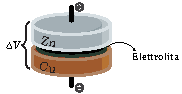
\includegraphics[width=0.35\textwidth]{images/chp5/chp5piladivolta.pdf}
	\end{center}
	Lo zinco sulla superficie dell'anodo è ossidato dalla soluzione elettrolitica e si dissolve nell'elettrolita come ioni carichi positiva, lasciando due elettroni liberi nel metallo.
	\begin{equation*}
		\text{anodo (ossidazione)}\colon \mathrm{Zn}\to\mathrm{Zn}^{2+}+2\mathrm{e}^{-}
	\end{equation*}
	Quando lo zinco entra nell'elettrolite, due atomi positivi di idrogeno dell'elettrolite accettano due elettroni dalla superficie dal catodo di rame, riducendoci ad una molecola di idrogeno non carica.
	\begin{equation*}
		\text{catodo (riduzione)}\colon2\mathrm{H}^{+}+2\mathrm{e}^{-}\to\mathrm{H}_2
	\end{equation*}
	Gli elettroni usati nel rame per formare le molecole di ossigine provengono da un filo esterno che lo collega al disco di zinco; l'idrogeno prodotto nella riduzione si disperde in forma gassosa.

	Misurando la \ddp tra i dischi si osserva un valore fisso di circa $\SI{0,76}{\volt}$; se impilassimo più celle la differenza di potenziale aumenterebbe. Il valore della \ddp misurata dipende dalla coppia di metalli scelti.
\end{digressionwt}
% L'energia elettrica è una forma di energia più "nobile", che si trasforma bene in altre forme di energia come il calore, ma che si ottiene difficilmente da altre forme, come dal calore o da reazioni chimiche, senza notevole dispersione di energia.
\subsection{Intensità di corrente}
\begin{define}[Intensità di corrente]
	L'\textbf{intensità di corrente elettrica}\index{intensità di corrente elettrica} è definita come la rapidità con cui fluiscono delle cariche attraverso una certa superficie $\Sigma$:
	\begin{equation}
		\tcboxmath[colback=yellowpastellow!30!white,colframe=ceruleancrayola!85!black,drop fuzzy shadow, nobeforeafter, math upper, tcbox raise base, enhanced]{I=\lim_{\Delta t}\frac{\Delta q}{\Delta t}=\dv{q}{t}}
	\end{equation}
\end{define}
\begin{attention}
	La corrente viene studiata per ragioni storiche supponendo che a muoversi siano \textit{cariche positive}, anche se nella maggior parte dei materiali che conducono corrente elettrica (ad esempio, i metalli) la corrente è portata da \textit{cariche negative}.
\end{attention}
\begin{define}[Velocità di deriva]
	La \textbf{velocità di deriva}\index{velocità!di deriva} è la \textit{velocità media} che hanno $N$ particelle cariche in un materiale a causa di un campo elettrico $\vba{E}$:
	\begin{equation}
		\tcboxmath[colback=yellowpastellow!30!white,colframe=ceruleancrayola!85!black,drop fuzzy shadow, nobeforeafter, math upper, tcbox raise base, enhanced]{\vba{v}_d=\frac{1}{N}\sum_{i=1}^{N}\vba{v}_i}
	\end{equation}
	La velocità di deriva ha la stessa direzione del campo elettrico.
\end{define}
I concetti di \textit{velocità di deriva} e \textit{intensità di corrente}, come possiamo facilmente immaginare, sono strettamente correlati.\\
\begin{minipage}{0.65\textwidth}
	 Consideriamo un filo conduttore percorso da portatori di carica positiva $+e$: essendo in presenza di una forza elettromotrice - e quindi di un campo elettrico - le cariche si muovono mediamente con velocità di deriva $\vba{v}_d$ e percorreranno, in un intervallo infinitesimo di tempo $\Delta t$, un tratto di filo
	\begin{equation*}
		d=\abs{\vba{v}_d}\Delta t
	\end{equation*}
\end{minipage}\hspace{5pt}
\begin{minipage}{0.34\textwidth}
	\begin{center}
		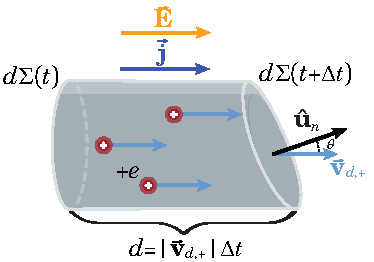
\includegraphics[width=1\textwidth]{images/chp5/chp5correntecavo1.pdf}
	\end{center}
\end{minipage}\\
La carica complessiva che passa attraverso una superficie infinitesima $d\Sigma$ in un tempo $\Delta t$ è quella contenuta in $\Delta V$, che corrisponde al volume di un cilindro infinitesimo di basi $d\Sigma\vba{u_n}\vdot\vbh{u}_d$ e altezza $d$, dove $\vba{u}_n$ è il versore normale alle superficie e $\vbh{u}_d$ è il versore nella direzione e verso della velocità di deriva:
\begin{align*}
	dV&=d\Sigma\vba{u_n}\vdot\vbh{u}_d d=\\
	&=d\Sigma\vba{u_n}\vdot\vbh{u}_d \abs{\vba{v}_d}\Delta t\\
	&=d\Sigma\vba{u_n}\vdot\vba{v}_d \Delta t =\\
	&=d\Sigma\cos\theta\abs{\vba{v}_d}\Delta t
\end{align*}
\begin{align*}
	\Delta q&=n_{+}edV=n_{+}e d\Sigma\vba{u_n}\vdot\vba{v}_d \Delta t=\\
	&)n_{+}e  d\Sigma\cos\theta\abs{\vba{v}_d}\Delta t
\end{align*}
Qui $\theta$ è l'angolo tra i due versori, $n_{+}$ la densità di cariche positive liberi per unità di volume ed $e$ la carica delle particelle libere. La carica di corrente infinitesima è dunque
\begin{align*}
	dI=\frac{\Delta q}{\Delta t}&=n_{+}edV=n_{+}e d\Sigma\vba{u_n}\vdot\vba{v}_d=\\
	&=n_{+}e  d\Sigma\cos\theta\abs{\vba{v}_d}
\end{align*}
Semplifichiamo questa notazione introducendo il concetto di \textbf{densità di corrente}. 
\begin{define}[Densità di corrente]
	La \textbf{densità di corrente}\index{densità!di corrente} è il campo vettoriale che ad ogni punto in un conduttore associa un vettore, la cui direzione è la velocità di deriva delle cariche \textit{positive} in tal punto e il cui modulo è pari alla quantità di carica che attraversa in un unità di tempo un unità di area della sezione perpendicolare del conduttore in tal punto. In altre parole,
	\begin{equation}
		\tcboxmath[colback=yellowpastellow!30!white,colframe=ceruleancrayola!85!black,drop fuzzy shadow, nobeforeafter, math upper, tcbox raise base, enhanced]{\vba{j}=n_{+}e\vba{v}_d}
	\end{equation}
\end{define}
Riscrivendo,
\begin{equation*}
	dI=\vba{j}\vdot \vba{u_n}d\Sigma
\end{equation*}
da cui si ottiene che l'intensità di corrente attraverso una superficie finita $\Sigma$ è
\begin{equation}
	I=\int_{\Sigma}\vba{j}\vdot \vba{u_n}d\Sigma=\Phi_{\Sigma}(\vba{j})
\end{equation}\\
\begin{minipage}{0.65\textwidth}
	Se, come nei conduttori metallici, i portatori di carica (con carica $-e$) sono negativi, la velocità di deriva $\vba{v}_{d,-}$ ha stessa direzione del campo elettrico ma verso \textit{opposto}; la densità di corrente è invece nella stessa direzione del campo elettrico perché la carica è \textit{negativa}:
	\begin{equation}
		\vba{j}=-n_{-}e\vba{v}_{d,-}
	\end{equation}
\end{minipage}\hspace{5pt}
\begin{minipage}{0.34\textwidth}
	\begin{center}
		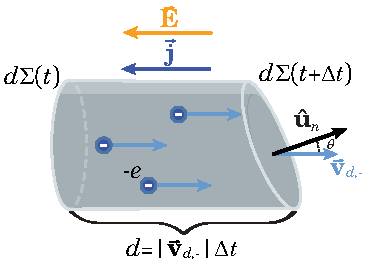
\includegraphics[width=1\textwidth]{images/chp5/chp5correntecavo2.pdf}
	\end{center}
\end{minipage}\\
\begin{minipage}{0.34\textwidth}
	\begin{center}
		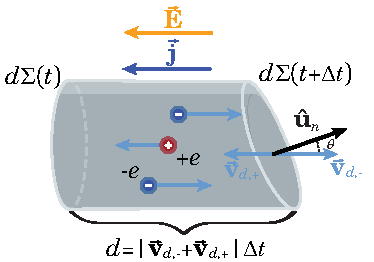
\includegraphics[width=1\textwidth]{images/chp5/chp5correntecavo3.pdf}
	\end{center}
\end{minipage}\hspace{5pt}
\begin{minipage}{0.65\textwidth}
	Se consideriamo invece \textit{fluidi ionizzati}, \textit{soluzioni elettrolitiche} o \textit{semiconduttori}, i portatori di carica sono di \textit{segno misto} e possono avere velocità di deriva differenti $\vba{v}_{d,+}$ e $\vba{v}_{d,-}$. In questi inusuali casi, la densità è ottenuta come una somma vettoriale di due quantità concorde che hanno lo stesso verso del campo elettrico:
	\begin{equation}
		\vba{j}=n_{+}e\vba{v}_{d,+}-n_{-}e\vba{v}_{d,-}
	\end{equation}
\end{minipage}
\paragraph{Unità di misura}
\begin{units}~\\
	\textbf{\textsc{Corrente elettrica:}} ampere ($\unit{\ampere}$).\\
	\textit{\textbf{Dimensioni:}} $[I]=\mathsf{I}$
\end{units}
\noindent L'\textbf{ampere}\index{ampere} - e non il \textit{coulomb}, come ci si potrebbe aspettare - è l'unica unità di misura fondamentale del SI che introdurremo in questa trattazione. Come precedentemente detto, $\SI{1}{\coulomb}$ è definito come la carica che una corrente da $\SI{1}{\ampere}$ attraversa una data superficie in $\SI{1}{\second}$.
Nella pratica sono utilizzati i suoi \textit{sottomultipli}, ad esempio:
\textit{sottomultipli}, ad esempio:
\begin{itemize}
	\item \textit{milliampere}: $\SI[per-mode = fraction,exponent-product=\ensuremath{\cdot}]{1}{\milli\ampere}=\SI[per-mode = fraction,exponent-product=\ensuremath{\cdot}]{e-3}{\ampere}$.
	\item \textit{microampere}: $\SI[per-mode = fraction,exponent-product=\ensuremath{\cdot}]{1}{\micro\ampere}=\SI[per-mode = fraction,exponent-product=\ensuremath{\cdot}]{e-6}{\ampere}$.
	\item \textit{nanoampere}: $\SI[per-mode = fraction,exponent-product=\ensuremath{\cdot}]{1}{\nano\ampere}=\SI[per-mode = fraction,exponent-product=\ensuremath{\cdot}]{e-9}{\ampere}$.
\end{itemize}
\begin{units}~\\
	\textbf{\textsc{Densità di corrente:}} ampere su metro quadro $\left(\unit[per-mode = fraction]{\ampere\per\square\meter}\right)$.\\
	\textit{\textbf{Dimensioni:}} $[j]=\dfrac{[I]}{[\Sigma]}=\mathsf{I}\mathsf{L}^{-2}$
\end{units}
\subsection{Conservazione della carica e l'equazione di continuità}
Data una densità $\vba{j}$, abbiamo trovato che la carica totale che passa nell'unità di tempo attraverso un volume $V$ è data dal flusso della densità tramite il bordo della $\Sigma$:
\begin{equation*}
	I=\int_{\Sigma}\vba{j}\vdot\vbh{u}_nd\Sigma
\end{equation*}
Sulla superficie, l'integrando $\vba{j}\vdot\vbh{u}_n$ \textit{non} ha necessariamente segno costante: dato che la direzione di $\vba{j}$ dipende dalla carica di deriva, segni diversi corrispondono a due situazioni differenti.
\begin{itemize}
	\item $\vba{j}\vdot\vbh{u}_n<0$: le cariche \textit{negative entrano} la superficie o le cariche \textit{positive escono}.
	\item $\vba{j}\vdot\vbh{u}_n>0$: le cariche \textit{negative escono} dalla superficie o le cariche \textit{positive entrano}.
\end{itemize}
Dal \textit{principio di conservazione della carica} nessuna carica nel conduttore (isolato) si può annichilire e sparire, e quindi la carica complessiva deve rimanere \textit{costante}. Se la carica interna $q_{int}$ alla superficie diminuisce, tale carica deve essere uscita dalla superficie e quindi è cambiata l'intensità di corrente $I$ che l'attraversa; in particolare, essa dovrà corrispondere alla \textit{variazione temporale} della \textit{carica interna}
\begin{equation}
	I=\int_{\Sigma}\vba{j}\vdot\vbh{u}_nd\Sigma=-\pdv{q_{int}}{t}
\end{equation}
Il \textit{meno} nell'espressione è dato dal fatto che se l'integrale è complessivamente positivo, ciò corrisponde ad una \textit{diminuzione} della carica interna - che ricordiamo si considera rispetto a quella positiva - e pertanto ha derivata negativa.\\
Se $V$ è il volume racchiuso da una superficie chiusa $\Sigma$, la carica interna è ovviamente
\begin{equation*}
	q_{int}=\int_V\rho dV
\end{equation*}
Possiamo derivare temporalmente entrambi i termini e scambiare integrale e derivata\footnote{Non motiveremo \textit{rigorosamente} perché si può fare questo scambio. Gli analisti che stanno leggendo questo testo si mettano il cuore in pace.} in quanto il volume è \textit{temporalmente invariante}.
\begin{equation*}
	\int_{\Sigma}\vba{j}\vdot\vbh{u}_nd\Sigma=-\pdv{q_{int}}{t}=-\pdv{t}\int_V\rho dt=-\int_V\pdv{\rho}{t} dV
\end{equation*}
Usando il \textit{teorema della divergenza} si ha dunque che
\begin{equation*}
	\int_V\div{\vba{j}}dV=-\int_V\pdv{\rho}{t} dV
\end{equation*}
Poiché tale relazione è vera per ogni volume $V$ si ha l'uguaglianze delle integrande, ottenendo così l'\textbf{equazione di continuità}\index{equazione!di continuità}:
\begin{equation}
	\tcboxmath[colback=yellowpastellow!30!white,drop fuzzy shadow, nobeforeafter, math upper, tcbox raise base, enhanced]{\div{\vba{j}}+\pdv{\rho}{t}=0}
\end{equation}
\begin{digression}
	Questa relazione vale in generale per descrivere il \textit{trasporto di una certa quantità conservata}, come l'energia e quantità di moto.
	Nello specifico, $\rho$ è l'ammontare della quantità per unità di volume (una \textit{densità}), mentre $\vba{j}$ è il flusso della quantità.\\
	Se la quantità \textit{non} si conserva, la legge si generalizza come
	\begin{equation}
		\div{\vba{j}}+\pdv{\rho}{t}=\sigma
	\end{equation}
dove $\sigma$ rappresenta quanta quantità viene \textit{generata} (se positiva) o \textit{rimossa} (se negativa) per unità di volume e di tempo.
\end{digression}
\paragraph{Il caso stazionario}
	Consideriamo il \textit{caso stazionario} dell'equazione di continuità, ossia quando la densità di carica $\rho$ risulta essere costante nel tempo. Dall'equazione di continuità segue  che
	\begin{equation*}
		\div{\vba{j}}=0
	\end{equation*}
	ossia la densità di corrente è un \textbf{campo solenoidale}\footnote{Nella ``Raccolta Differenziata'', a pag. \ref{CampoSolenoidale} è possibile trovare la definizione di campo solenoidale e altre proprietà.}. Consideriamo una porzione tubulare di conduttore come in figura.
	\begin{center}
		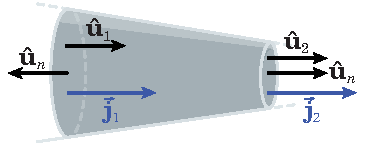
\includegraphics[width=0.35\textwidth]{images/chp5/chp5casostazionario.pdf}
	\end{center}
	Sappiamo che il flusso sulla superficie che delimita questa porzione è nullo, ma esso è determinato completamente dai flusso sulle sezioni perpendicolari del conduttore\footnote{La densità di corrente sulla superficie laterale del tubo è tangente e quindi il suo flusso è nullo.}
	\begin{equation*}
		0=\oint_{\Sigma}\vba{j}\vdot\vbh{u}_nd\Sigma=\int_{\Sigma_1}\vba{j}_1\vdot\vbh{u}_nd\Sigma_1+\int_{\Sigma_2}\vba{j}_2\vdot\vbh{u}_nd\Sigma_2
	\end{equation*}
	Definiamo $\vba{u}_i$ come il versore che indica la direzione del moto delle cariche tramite la superficie $\Sigma_i$. Se consideriamo le intensità di correnti lungo le sezioni...
	\begin{align*}
		I_1&\coloneqq\int_{\Sigma_1}\vba{j}_1\vdot\vbh{u}_1d\Sigma_1=-\int_{\Sigma_1}\vba{j}_1\vdot\vbh{u}_nd\Sigma_1\\
		I_2&\coloneqq\int_{\Sigma_2}\vba{j}_2\vdot\vbh{u}_2d\Sigma_2=\int_{\Sigma_2}\vba{j}_2\vdot\vbh{u}_nd\Sigma_1
	\end{align*}
	...allora segue che $0=I_1-I_2$, ossia
	\begin{equation}
			\tcboxmath[colback=yellowpastellow!30!white,drop fuzzy shadow, nobeforeafter, math upper, tcbox raise base, enhanced]{I_1=I_2}
	\end{equation}
Nel caso stazionario, l'intensità di corrente è \textit{sempre costante} - in tal caso si parla di \textbf{corrente stazionaria}\index{corrente elettrica!stazionaria}.
\begin{intuit}
	Riprendendo l'analogia con fluidodinamica tra intensità di corrente e portata, la portata è costante nei fluidi incomprimibili, cioè quelli la cui densità di massa è $\rho=\mathrm{const}$.
\end{intuit}
\begin{attention}
	Sebbene il termine \textit{stazionario} possa far pensare ad una situazione di immobilità, ciò non è più lontano dalla realtà! Anche nel caso stazionario le cariche sono in movimento - ed eccome se si muovono! - ma intendiamo che il flusso di cariche stia scorrendo praticamente da sempre, senza cambiamenti e senza accumulo di cariche in alcun luogo.
\end{attention}
\section{Legge di Ohm}
Ad inizio del capitolo, abbiamo descritto brevemente come sono costituiti i conduttori metallici. Tale descrizione, in realtà, corrisponde al \textbf{modello di Drude-Lorentz} della \textit{conduzione elettrica} proposto dal fisico tedesco \textbf{Paul Drude} (1863 – 1906) nel 1900 ed espanso nel 1905 dall'olandese \textbf{Hendrick Antoon Lorentz} (1853 – 1928).

Il modello permette di spiegare, nell'ambito della teoria classica dell'elettromagnetismo, le proprietà di trasporto degli elettroni nei materiali - in particolare i metalli - tramite la teoria cinetica: gli elettroni si comportano, secondo questa interpretazione, in modo molto simile ad un \textit{flipper}\footnote{Per gli amici d'oltreoceano o per coloro che si divertivano ai giochi di \textit{Windows XP}\texttrademark\ , un \textit{pinball}.}, in cui elettroni rimbalzanti \textit{urtano} continuamente contro un reticolo cristallini di ioni fissi.
\begin{digression}
	Tale modello fu integrato nel 1933 da \textbf{Arnold Sommerfeld} (1868 – 1951) e \textbf{Hans Bethe} (1906 – 2005) con i risultati della teoria quantistica nel \textbf{modello di Drude-Sommerfeld}.\\
	Una differenza, ad esempio, è che il modello \textit{non parla} esplicitamente di ioni o di reticoli cristallini: tale assenza viene giustificata in termini quantistici.
\end{digression}
\begin{minipage}{0.38\textwidth}
	\begin{center}
		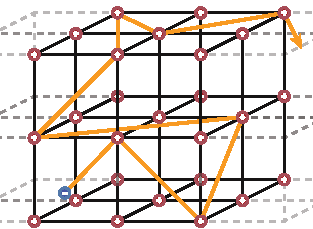
\includegraphics[width=1\textwidth]{images/chp5/chp5reticolocristallino.pdf}
	\end{center}
\end{minipage}\hspace{5pt}
\begin{minipage}{0.61\textwidth}
	Approfondiamo meglio questo modello. Gli elettroni liberi si muovono attraverso il reticolo cristallino in modo \textit{completamente disordinato}; nel loro moto, gli elettroni si vanno a scontrare continuamente con gli ioni in interazioni che chiamiamo \textit{urti}. Tra un urto e il successivo il moto è libero e in \textit{traiettoria rettilinea}, cosicché il moto degli elettroni si possa rappresentare come un \textit{spezzata} di segmenti con direzione e verso variabili. Senza campo elettrico \textit{non} c'è una direzione privilegiata e quindi una corrente.
\end{minipage}\\
Si può definire
\begin{itemize}
	\item un \textbf{tempo medio di percorrenza} $\tau$.
	\item un \textbf{cammino libero medio} $\mathcal{l}$ tra due urti successivi
\end{itemize}
che sono legati tra di loro dalla velocità media $v$ degli elettroni nel metallo.
\begin{equation}
	\mathcal{l}=v\tau
\end{equation}
Da queste supposizioni microscopiche possiamo derivare una \textit{legge macroscopica}.\\
\begin{minipage}{0.38\textwidth}
	\begin{center}
		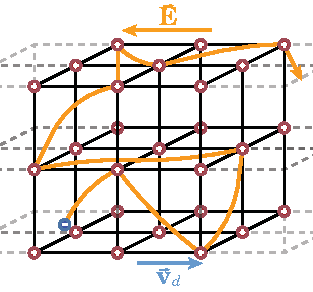
\includegraphics[width=1\textwidth]{images/chp5/chp5reticolocristallinoacc.pdf}
	\end{center}
\end{minipage}\hspace{5pt}
\begin{minipage}{0.61\textwidth}
	 All'applicazione di un campo elettrico $\vba{E}$ non si muoverà più di moto rettilineo uniforme, ma subisce un \textit{accelerazione}
	\begin{equation*}
		\vba{a}=\frac{\vba{F}}{m_{e}}=-\frac{e}{m_{e}}\vba{E}
	\end{equation*}
	dove $m_e$ è la massa dell'elettrone. Alla distribuzione casuale delle velocità si sovrappone quindi una velocità data da questa accelerazione; poiché è più piccola rispetto a quella che l'elettrone possiede di per sé, il tempo medio $\tau$ non cambia in modo significativo.
\end{minipage}\\
 Se $\vba{v}_i$ è la velocità dopo un urto, la velocità subito prima l'urto successivo sarà
\begin{equation*}
	\vba{v}_{i+1}=\vba{v}_i-\frac{e}{m_{e}}\vba{E}\tau
\end{equation*}
Calcoliamo la velocità media su $N$ elettroni, con $N$ molto grande, in modo da definire la \textit{velocità di deriva} indotta dal campo elettrico:
\begin{equation*}
	\vba{v}_d=\frac{1}{N}\sum_{i=1}^{N}\vba{v}_{i+1}=\frac{1}{N}\sum_{i=1}^{N}\vba{v}_i-\frac{e}{m_{e}\tau}\vba{E}=\left<\vba{v}\right>-\frac{e}{m_{e}\tau}\vba{E}
\end{equation*}
La media delle velocità dopo l'urto è casuale e perciò è nulla; la velocità di deriva è quindi
\begin{equation}
	\vba{v}_d=-\frac{e\tau}{m_{e}}\vba{E}
\end{equation}
Se $n_{-}$ la densità di elettroni liberi per unità di volume, la densità di corrente che consegue a questo modo ordinato è
\begin{equation}
	\vba{j}=-n_{-}e\vba{v}_d=\frac{n_{-}e^2\tau}{m_{e}}\vba{E}=\sigma\vba{E}
\end{equation}
dove
\begin{equation*}
	\sigma=\frac{n_{-}e^2\tau}{m_{e}}
\end{equation*}
è una grandezza caratteristica del materiale nota come \textbf{conduttività}.
L'equazione
\begin{equation}
	\tcboxmath[colback=yellowpastellow!30!white,drop fuzzy shadow, nobeforeafter, math upper, tcbox raise base, enhanced]{\vba{j}=\sigma\vba{E}}
\end{equation}
è nota come \textbf{legge di Ohm della conduzione elettrica}\index{legge!di Ohm}, dal fisico tedesco Georg \textbf{Ohm} che nel 1827 introdusse un caso specifico di tale equazione per spiegare dei risultati sperimentali da lui studiati. La legge si può scrivere anche nella forma
\begin{equation}
	\tcboxmath[colback=yellowpastellow!30!white,drop fuzzy shadow, nobeforeafter, math upper, tcbox raise base, enhanced]{\vba{E}=\rho\vba{j}}
\end{equation}
dove
\begin{equation*}
	\rho=\frac{1}{\sigma}
\end{equation*}
è detta \textbf{resistività}.
\begin{define}[Conduttività e resistività]
	La \textbf{conduttività}\index{conduttività} è una grandezza associata ai conduttori definita come
	\begin{equation}
		\tcboxmath[colback=yellowpastellow!30!white,colframe=ceruleancrayola!85!black,drop fuzzy shadow, nobeforeafter, math upper, tcbox raise base, enhanced]{\sigma=\frac{n_{-}e^2\tau}{m_{e}}}
	\end{equation}
	che rappresenta la difficoltà della corrente a muoversi nel conduttore ed è caratteristica del \textit{materiale} con cui è fatto.\\
	Il valore
	\begin{equation}
		\tcboxmath[colback=yellowpastellow!30!white,colframe=ceruleancrayola!85!black,drop fuzzy shadow, nobeforeafter, math upper, tcbox raise base, enhanced]{\rho=\frac{1}{\sigma}}
	\end{equation}
	viene detto \textbf{resistività}\index{resistività} e rappresenta la difficoltà della corrente a muoversi nel conduttore.
\end{define}
\textit{Non tutti} i conduttori rispettano questa legge, ma soltanto quelli che sono detti \textbf{conduttori ohmici}\index{conduttore!ohmico}.
\begin{exampleswt}[Esempi di conduttori ohmici e non ohmici]~
	\begin{itemize}
		\item \textbf{Ohmici:} fili conduttori di metalli come rame, o argento, resistenze ideali.
		\item \textbf{Non ohmici:} filamento di tungsteno delle lampade a incandescenza, diodi, semiconduttori.
	\end{itemize}
\end{exampleswt}
\subsection{Legge di Ohm nei conduttori metallici}
Consideriamo un conduttore metallico cilindrico di lunghezza $d=\overline{AB}$ e sezione $\Sigma$. Ai capi del conduttore è applicata, con un generatore di \fem, una \ddp pari a
\begin{equation*}
	V=V_A-V_B=\int_{A}^{B}\vba{E}\vdot d\vba{s}=Ed>0
\end{equation*}
Il campo elettrico è costante (con modulo $|\vba{E}|=E$) e diretto, parallelo all'asse del cilindro, da $A$ verso $B$; in regime stazionario, anche la densità di corrente $\vba{j}$ è costante (con modulo $\abs{\vba{j}}=j$) e scorre nella stessa direzione\footnote{Ciò è dovuto alla scelta storica di orientare la densità di corrente con le cariche positive. Gli elettroni, invece, percorrono il conduttore da $B$ verso $A$.}. Allora, dalla \textit{legge di Ohm}, segue che
\begin{equation*}
	I=\int_{\Sigma}\vba{j}\vdot\vbh{u}_nd\Sigma=j\Sigma=\sigma E\Sigma=\frac{V}{d}\sigma\Sigma=V\frac{\Sigma}{\rho d}
\end{equation*}
Definita la \textbf{resistenza} come
\begin{equation*}
	R=\frac{\rho d}{\Sigma}
\end{equation*}
si ottiene la \textbf{legge di Ohm}\index{legge!di Ohm} nella forma amata dagli elettrotecnici:
\begin{equation}
	\tcboxmath[colback=yellowpastellow!30!white,colframe=ceruleancrayola!85!black,drop fuzzy shadow, nobeforeafter, math upper, tcbox raise base, enhanced]{V=IR}
\end{equation}
La legge si può scrivere anche nella forma
\begin{equation}
	\tcboxmath[colback=yellowpastellow!30!white,colframe=ceruleancrayola!85!black,drop fuzzy shadow, nobeforeafter, math upper, tcbox raise base, enhanced]{I=GV}
\end{equation}
dove
\begin{equation*}
	G=\frac{1}{R}
\end{equation*}
è detta \textbf{conduttanza}.
\begin{define}[Resistenza e conduttanza]
	La \textbf{resistenza}\index{resistenza} è una grandezza associata ai conduttori metallici di lunghezza $d$ e sezione $\Sigma$, definita come
	\begin{equation*}
		\tcboxmath[colback=yellowpastellow!30!white,colframe=ceruleancrayola!85!black,drop fuzzy shadow, nobeforeafter, math upper, tcbox raise base, enhanced]{R=\frac{\rho d}{\Sigma}}
	\end{equation*}
	che rappresenta la \textit{difficoltà} della corrente a muoversi nel conduttore. Il termine $\rho$ è la \textit{resistività} del conduttore e dipende dal materiale.\\
	Il valore
	\begin{equation}
			\tcboxmath[colback=yellowpastellow!30!white,colframe=ceruleancrayola!85!black,drop fuzzy shadow, nobeforeafter, math upper, tcbox raise base, enhanced]{G=\frac{1}{R}}
	\end{equation}
	viene detto \textbf{conduttanza}\index{conduttanza} e rappresenta la facilità della corrente a muoversi nel conduttore.
\end{define}
\paragraph{Unità di misura}
\begin{units}\index{ohm}~\\
	\textbf{\textsc{Resistenza elettrica:}} ohm ($\unit{\ohm}$) o volt su ampere $\left(\unit[per-mode = fraction]{\volt\per\ampere}\right)$.\\
	\textit{\textbf{Dimensioni:}} $[R]=\dfrac{[V]}{[I]}=\mathsf{M} \mathsf{L}^2  \mathsf{T}^{-3}\mathsf{I}^{-2}$
\end{units}
\begin{units}\index{siemens}~\\
	\textbf{\textsc{Conduttanza elettrica:}} siemens ($\unit{\siemens}$), mho  ($\mho$) o ampere su volt $\left(\unit[per-mode = fraction]{\ampere\per\volt}\right)$.\\
	\textit{\textbf{Dimensioni:}} $[G]=\dfrac{[I]}{[V]}=\mathsf{I}^{2}\mathsf{T}^{3}\mathsf{M}^{-1} \mathsf{L}^{-2}$
\end{units}
\begin{digressionwt}[\textit{E mho il siemens?} Tragicommedia in tre atti sulla conduttanza]
	Nei libri di testo contemporanei l'unità di misura associata alla conduttanza è il \textit{siemens}; tuttavia, in alcuni un po' datati è possibile trovare l'alquanto buffo \textit{mho}. Inoltre, se scartabellassimo libri ancora più vecchi troveremmo sì il \textit{siemens}, ma per indicare la resistenza! Che pasticcio hanno combinato i fisici con questa grandezza?\newline~\\
	Facciamo un po' d'ordine e torniamo indietro al 1860. L'ingegnere Werner Siemens era tra i proprietari di un'azienda che costruiva telegrafi in Germania, Russia e Regno Unito; per migliorare il loro funzionamento aveva bisogno di studiare a livello pratico la resistenza dei conduttori al passaggio della corrente, ma una buona unità di misura di tale grandezza, che sia riproducibile, non esisteva. Siemens propose lui stesso negli \textit{Annalen der Physik und Chemie} quella che diventerà nota come \textit{l'unità di mercurio del Dr. Siemens}: essa corrispondeva alla resistenza elettrica presente in una colonna di mercurio con lunghezza di un metro e sezione uniforme di $\SI{1}{\milli\metre\squared}$ mantenuta alla temperatura di zero gradi Celsius.\\
	Tale unità --- il cui nome completo ha quel non so che di cinema espressionista tedesco e potrebbe figurare bene come pellicola accanto a \textit{Il gabinetto del dottor Caligari} --- verrà semplicemente chiamata \textit{siemens}, nome che non causerà assolutamente alcuna confusione in futuro.\\
	Seppur sia simile, almeno concettualmente, ad altre unità basate sul mercurio come l'\textit{atmosfera}, in realtà si rivelò problematica proprio nel suo tentativo di essere riproducibile: per definire questa colonna di mercurio erano necessari dei tubi di vetro, i quali però non avevano sezioni costanti. Altri fattori come pressione dell'aria, umidità... potevano influenzare questa misurazione. Inoltre, non era coerente con altre unità di misura preesistenti! Nonostante questi problemi, fu comunque utilizzata per diversi anni.\newline~\\
	La ricerca di un'unità di misura migliore proseguì. L'anno successivo, il 1861, Latimer Clark e Sir Charles Bright presentarono un articolo all'\textit{Associazione Britannica per l'Avanzamento della Scienza}, suggerendo di creare uno standard per la resistenza e di chiamarla in onore del fisico tedesco Georg Ohm... chiamandola \textit{ohma}. Si stabilì subito una commissione, a cui parteciparono fisici dal calibro di James Clark Maxwell e Lord Kelvin, per inventare un unità che fosse coerente con il sistema metrico francese e pratica da utilizzare - a differenza di quella di Siemens.
	Nel terzo verbale della commissione, nel 1864, si riproposte di chiamarla in onore di Ohm e dunque si riferirono all'unità di misura come... \textit{ohmad}. A volte mi chiedo se i fisici ci sono o ci fanno. Solo nel 1867 il termine \textit{ohm} si userà in modo diffuso.
	
	A dir la verità, l'\textit{ohm} definito dall'Associazione Britannica non era neanche così differente da quello di Siemens, dato che cambiava soltanto la lunghezza della colonna di mercurio da $\SI{100}{\centi\meter}$ a $\SI{104.7}{\centi\meter}$. Ciò nonostante, dato che avere due unità di misura differenti per una stessa grandezza era ridicolo, nel 1881 al \textit{Congresso Internazionale degli Elettricisti} si decise di compiere una scelta definitiva tra le due: l'unità di misura della resistenza non doveva essere il \textit{siemens}, ma l'\textit{ohm}... anche se nel frattempo la colonna di mercurio si allungò a $\SI{104.9}{\centi\meter}$.\newline
	
	\noindent Come ricordò Maxwell al convegno, ``le dimensioni contano\textsuperscript{[Senza fonte]}
	%\textsuperscript{{$\left[\parbox{15em}{\tiny\textit{Fonte: Maxwell ``Manualotso'', un mercoledì pranzo, in un anonimo 100Montaditos}}\right]$}}
	 '' e negli anni l'unità di misura rimase la stessa, ma la colonnina di mercurio cambiò lunghezza più e più volte per adattarsi a studi sempre più analitici - stranamente non cambio lo spessore, ma evidentemente quello non contava più di tanto. La colonna di mercurio puro rimase lo standard fino alla \textit{Conferenza Generale sui Pesi e le Misure} del 1948, dove l'\textit{ohm} fu ridefinito in termini assoluti. Attualmente, il \textit{siemens} di Siemens vale circa $\SI{0.9537}{\ohm}$ moderni.
	
	Il povero Siemens, nonostante l'unità della resistenza non prese il suo nome, non si perse d'animo e continuò a sperimentare con l'elettromagnetismo: nel 1867 brevettò una delle prime dinamo industriali --- casualmente lo stesso giorno in cui Sir Charles Wheatstone brevettò una sua personale versione della dinamo. Successivamente, nel 1888 divenne nobile, trasformando il suo cognome in \textit{von Siemens}, e negli anni a seguire la sua azienda si espanse fino a diventare l'odierna multinazionale \textit{Siemens AG}.\newline~\\
	La resistenza elettrica aveva finalmente ottenuto un'unità di misura, ma ne mancava ancora una per la \textit{conduttanza}. O meglio, siccome tale grandezza era il reciproco della resistenza, mancava soltanto il nome dell'unità di misura: dopotutto, se i reciproci dei \textit{secondi} si chiamano \textit{hertz}, anche il reciproco della resistenza merita un nome, che diamine!
	
	Il primo ad accorgersi di cotale mancanza fu Lord Kelvin. Basandosi su alcune idee fornitegli dai suoi studenti,  nel 1883 Lord Kelvin propose al grande pubblico di utilizzare il termine \textit{mho}.	Se non ve ne foste accorti, \textit{mho} è letteralmente \textit{ohm} letto al contrario - perché un \textit{mho} è il reciproco di un \textit{ohm}.\\
	Non fu l'unica proposta avanza in quell'incontro: Kelvin propose entusiasta - sempre su un idea di origine studentesca - che la corretta pronuncia di \textit{mho} si dovesse ottenere prendendo una registrazione di \textit{ohm} con il fonografo di Edison e ascoltandola al contrario.\\
	Non si sa se Kelvin non si accorse di essere stato preso in giro dagli studenti o Kelvin stava cercando di prendersi gioco del suo pubblico, ma sta di fatto che \textit{mho} prese inesplicabilmente piede come nome per la conduttanza; anche il simbolo del \textit{mho} fu ottenuto ribaltando la Omega maiuscola dell'\textit{ohm}.

	La cosa peculiare è che la malsana idea venne riproposta in elettrotecnica in altri due contesti.
	\begin{itemize}
		\item l'ingegnere Arthur E. Kennelly scelse il \textit{daraf} per descrivere l'\textit{elastanza elettrica}, in quanto essa è il reciproco della conduttanza e la conduttanza usa i \textit{farad}. In questo caso mi turba di più il nome dell'inverso della conduttanza che non il \textit{daraf}.
		\item l'ingegnere Vladimir Karapetoff propose nel 1911 di usare gli \textit{yrneh} come reciproco dell'unità di misura dell'induttanza, l'\textit{henry}; la pronuncia, tra l'altro, doveva essere ``earney''. Non dormo la notte cercando di capire come mai quella sia la pronuncia di \textit{yrneh}.
	\end{itemize}
	Saltiamo molti anni e nella \textit{Conferenza Generale sui Pesi e le Misure} 1971 si decise che questo scherzo era durato abbastanza: l'unità di misura della conduttanza verrà chiamato \textit{siemens}... aspettate, \textit{di nuovo siemens}?\\
	Eh sì, gli scienziati lì riuniti volevano dedicare un unità di misura a Siemens --- non hanno neanche specificato se a Werner von Siemens o al fratello Sir William Siemens --- senza tener conto che in passato è stata usata un'unità di misura dallo stesso nome per tutt'altri scopi. Non si curarono di questo e il \textit{siemens} fu approvato: da allora, usare il \textit{mho} per la conduttanza è considerato un nome non accettabile (e non consono) per un'unità di misura del SI e pertanto deve essere rigorosamente evitato.
\end{digressionwt} 
\section{Potenza dissipata da una resistenza}
In un conduttore elettrico in cui scorre una corrente elettrica, la \textbf{potenza} necessaria per spostare una carica è data da
\begin{equation}
	P=\pdv{W}{t}=\vba{F}\vdot \vba{v}_d=e\vba{E}\vdot\vba{v}_d
\end{equation}
Questa energia viene dispersa nell'ambiente sotto forma di \textit{calore}.\\
Se $n$ è il numero di cariche per unità di volume, la \textbf{densità di potenza}, ossia la potenza per unità di volume, è
\begin{equation}
	P_V=ne\vba{E}\vdot\vba{v}_d=\vba{j}\vdot \vba{E}
\end{equation}
con $\vba{j}$ la densità di corrente. La potenza totale dissipata segue facilmente da
\begin{equation}
	P=\int_{V}P_VdV
\end{equation}
Consideriamo il caso particolare di un conduttore ohmico cilindrico di lunghezza $d$ e di superficie $\Sigma$ in situazione di corrente stazionaria. La densità di corrente e il campo elettrico sono costanti e paralleli, dunque densità di potenza è costante e pari a
\begin{equation}
	P_V=jE
\end{equation}
quindi la potenza totale è data da
\begin{equation*}
	P=\int_{V}P_VdV=P_V\mathcal{Vol}=jE\Sigma d=\underbrace{\Sigma j}_{=I}\cdot\underbrace{Ed}_{=V}=IV
\end{equation*}
dove $V$ è il calo di potenziale ai capi del conduttore. In sostanza, in presenza di un calo di potenziale si ha una dispersione di energia sotto forma di calore: maggiore è la corrente nel conduttore, maggiore sarà l'energia dispersa.

Cosa succede, a livello microscopico? La \ddp ai capi del conduttore generano un campo elettrico che induce una velocità di deriva nei portatori di carica, fornendo a loro un'energia cinetica. Quando le particelle urtano gli ioni del reticolo cristallino, nell'urto (elastico) viene ceduta energia cinetica dagli elettroni agli ioni, i quali tuttavia sono immobili e quindi \textit{vibrano}, trasformando quella energia sotto forma di calore. Quanta energia viene dispersa dipende dal materiale e dalla geometria del conduttore: questa informazione fisico-empirica è presentata matematicamente nella resistività $\rho$ e, di conseguenza, dalla resistenza.

Questo è quello che viene chiamato \textbf{effetto Joule}\index{effetto Joule}; nella sua forma più basica questo si esprime dalla legge
\begin{equation}
	\tcboxmath[colback=yellowpastellow!30!white,drop fuzzy shadow, nobeforeafter, math upper, tcbox raise base, enhanced]{P=IV}
\end{equation}
Se assumiamo che il conduttore trasforma completamente l'energia in calore, allora
\begin{equation}
	\tcboxmath[colback=yellowpastellow!30!white,drop fuzzy shadow, nobeforeafter, math upper, tcbox raise base, enhanced]{P=IV=I^2R=\frac{V^2}{R}}
\end{equation}
\begin{example}
	Qualunque elettrodomestico o oggetto che produce calore, in una forma o nell'altra, a partire da corrente elettrica si basa sull'effetto Joule, come lampadine, fon, forni...
\end{example}
\begin{observe}
	La legge dell'effetto Joule si può utilizzare per descrivere il legame tra la potenza generata da un generatore di \fem e la corrente in un conduttore: se $\mathcal{E}$ è la forza elettromotrice generata e $P$ la potenza prodotta dal generatore, il generatore produrrà una corrente di intensità
	\begin{equation}
		I=\frac{P}{\mathcal{E}}
	\end{equation}
\end{observe}
\paragraph{Lavoro compiuto dal campo elettrico}
Per ottenere l'energia dispersa in un periodo di tempo $t$, ossia il lavoro compiuto dal campo elettrico nel conduttore per spostare le cariche, ci basta integrare rispetto al tempo la potenza:
\begin{equation}
	U=W=\int_{0}^{t}Pdt=\int_{0}^t IVdt
\end{equation}
Se la corrente è stazionaria, si ha
\begin{equation}
	U=W=\frac{I^2V}{2}=\frac{I^3R}{2}=\frac{V^3}{2R^2}
\end{equation}
\section{Forza elettromotrice}\label{femxesteso}
A pag. \pageref{fem} abbiamo accennato ai \textbf{generatori di forza elettromotrice}\index{generatore!di forza elettromotrice} (\fem), dispositivi che trasforma energia \textit{non} elettrica in energia elettrica tale da mantenere, ai capi del generatore, una differenza di potenziale $\Delta V$, \textit{indipendentemente} da cosa ci si collega.

Come abbiamo visto, il passaggio di corrente implica un trasferimento di energia dalla corrente circolante ad altre forme - ad esempio, calore per \textit{effetto Joule}, oppure sotto forma di energia meccanica, ecc... Di conseguenza, il generatore è l'elemento che deve rifornire con continuità tale energia, a mano a mano che essa viene dissipata o trasformata.

Preso un generatore di \fem con dei fili attaccati, in essi possiamo incontrare le cariche elettriche in due situazioni differenti: alcune sono in movimento, creando così una corrente elettrica, altre sono accumulate ai capi del generatore. Sono quest'ultime che effettivamente causano la differenza di potenziale e sono sorgente di un campo elettrostatico $\vba{E}_s$ che mantiene la corrente stazionaria. Le cariche accumulate non sono sempre le stesse, bensì le cariche libere \textit{provengono} da esse: il generatore, pertanto, deve continuamente ripristinarle in qualche maniera per mantenere un flusso costante su tutto il filo.

Se supponiamo di prendere un filo conduttore che collega entrambi i capi del generatore di \fem, il flusso di cariche è \textit{costante} su tutto il \textit{circuito} $\gamma$ e sull'intero filo deve esserci un campo elettrico $\vba{E}$ adeguato per produrre il movimento di cariche. Poiché lungo il circuito l'energia delle cariche viene trasformata in parte in altre forme di energia, il lavoro fornito dal campo elettrico \textit{totale} $\vba{E}$ agente sui portatori di carica lungo l'intero filo deve essere diverso da zero - in caso contrario, non si potrebbe mantenere costante l'intensità di corrente!
\begin{equation*}
	\oint_{\gamma}\vba{E}\vdot d\vba{s}\neq 0
\end{equation*}
È evidente che $\vba{E}$ non può essere conservativo. Poichè $\vba{E}_s$, causato dagli accumuli di carica, è conservativo, è necessario immaginare la presenza di un campo elettrico \textit{non} conservativo $\vba{E}_f$ prodotto \textit{all'interno} del generatore e che si oppose a $\vba{E}_s$. Tale campo, che chiameremo \textbf{campo elettromotore}\index{campo!elettromotore}, separa le cariche ai capi del generatore e le spinge ai capi opposti - $\vba{E}_f$ ha verso opposto a $\vba{E}_s$.
\begin{digression}
	In realtà, $\vba{E}_f$ è la manifestazione esterna di azioni di natura \textit{non elettrostatiche} che tuttavia intervengono sulle cariche del generatore.
\end{digression}
Possiamo ora associare al generatore la \textbf{forza elettromotrice}.
\begin{define}[Forza elettromotrice]
	La forza elettromotrice (\fem) del generatore è la quantità
	\begin{equation}
		\tcboxmath[colback=yellowpastellow!30!white,colframe=ceruleancrayola!85!black,drop fuzzy shadow, nobeforeafter, math upper, tcbox raise base, enhanced]{f=\int_{\gamma}\vba{E}_f\vdot d\vba{s}=\int_{B}^{A}\vba{E}_f\vdot d\vba{s}}\label{femRistretta}
	\end{equation}
	dove $\gamma$ è un cammino \textit{interno} al generatore dal capo negativo $B$ al capo positivo $A$.
\end{define}
La forza elettromotrice rappresenta dunque il lavoro eseguito dal campo elettromotore per portare una carica negativa da un capo all'altro del generatore, al suo interno.
\begin{observe}
	A discapito del nome, la forza elettromotrice \textit{non} è una forza, bensì è un \textit{lavoro per unità di carica}:
	\begin{equation*}
		\left[f\right]=\left[E\right]\left[\gamma\right]=\frac{\unit{\volt}}{\Ccancel[red]{\unit{\meter}}}\Ccancel[red]{\unit{\meter}}=\unit{\volt}
	\end{equation*}
\end{observe}
\paragraph{La forza elettromotrice come differenza di potenziale}
Nella pratica non è possibile calcolare la forza elettromotrice con la definizione che abbiamo fornito. Tuttavia, possiamo ricondurci alla \fem espressa come differenza di potenziale ai capi del generatore.

Possiamo supporre che nella fase iniziale di funzionamento del generatore, il campo elettromotore $\vba{E}_f$ cerchi lui stesso di accumulare cariche ai capi del generatore; in questo modo, esso genera al contempo un campo elettrostatico $\vba{E}_s$ ad esso contrario, via via crescente fino alla situazione di equilibrio per cui, all'interno del generatore, si ha $\vba{E}_f=-\vba{E}_s$. Ne segue che
\begin{equation*}
	f=\int_{B}^{A}\vba{E}_f\vdot d\vba{s}=\int_{B}^{A}\left(-\vba{E}_s\right)\vdot d\vba{s}=\int_A^B\vba{E}_s\vdot d\vba{s}=\int_A^B\left(-\grad{V}\right)\vdot d\vba{s}=\eval{-V}_A^B=V_A-V_B
\end{equation*}
dove abbiamo utilizzato il fatto che $\vba{E}_s$ è conservativo.

La precedente definizione di forza elettromotrice può essere generalizzata all'intero circuito se non è possibile circoscrivere in una delimitata zona il \textbf{campo elettromotore}:
\begin{equation}
	\tcboxmath[colback=yellowpastellow!30!white,drop fuzzy shadow, nobeforeafter, math upper, tcbox raise base, enhanced]{f=\oint \vba{E}_f\vdot d\vba{s}}\label{femGeneralizzata}
\end{equation}
La \eqref{femGeneralizzata} si riduce alla \eqref{femRistretta} se $\vba{E}_f$ è localizzato solo lungo un certo tratto $\gamma$ del circuito. Ancor più in generale vale per il campo elettrico \textit{totale} $\vba{E}$ la legge
\begin{equation}
	\tcboxmath[colback=yellowpastellow!30!white,drop fuzzy shadow, nobeforeafter, math upper, tcbox raise base, enhanced]{f=\oint \vba{E}\vdot d\vba{s}}
\end{equation}
dato che il contributo di $\vba{E}_s$ al lavoro di $\vba{E}$ è nullo essendo conservativo.
\section{Circuiti elettrici}
\begin{define}[Circuito elettrico]
	Un \textbf{circuito elettrico}\index{circuito} è un insieme interconnesso di componenti elettrici, connessi da fili conduttori in un percorso chiuso in modo che la corrente elettrica possa fluire con continuità.
\end{define}
\begin{define}[Componente, nodo, ramo, maglia, interruttore]
	In un circuito elettrico,
	\begin{itemize}
		\item un \textbf{componente elettrico}\index{componente elettrico} è un congegno con due o più terminali da cui la corrente può entrare o uscire allo scopo di modificare il comportamento degli elettroni o dei campi elettromagnetici. Esse si distinguono in
		\begin{enumerate}
			\item[$\bullet$] componenti \textbf{attive}: dette anche \textbf{sorgenti}\index{sorgenti} o \textit{generatori}, producono energia elettrica in quanto indicono una corrente o una \ddp per mezzi non elettrici; ad esempio, sono componenti attive i generatori di tensore e di corrente.
			\item[$\bullet$] componenti \textbf{passive}: non producono energia, bensì la ricevono per utilizzarla in altri scopi; ad esempio, sono componenti passive  i condensatori, i resistori e gli induttori. 
		\end{enumerate}
		\item un \textbf{nodo}\index{nodo} è il punto di incontro di tre o più fili.
		\item un \textbf{ramo}\index{ramo} è un filo con e/o componenti che collegano due nodi 
		\item una \textbf{maglia}\index{maglia} è un insieme di rami all'interno di un circuito che forma un circuito chiuso senza auto-intersezioni.
		\item un \textbf{interruttore}\index{interruttore} permette di chiudere o aprire un circuito, lasciando rispettivamente passare o fermando la corrente elettrica.
	\end{itemize}
\end{define}
Lo scopo dell'\textbf{analisi dei circuiti elettrici} è quella di \textit{risolvere} i circuiti, ossia trovare le differenze di potenziali e le correnti per ciascuna componente del circuito. Ovviamente, noi studieremo soltanto un \textit{modello} dei circuiti elettrici reali, supponendo che:
\begin{itemize}
	\item La corrente si suppone \textit{stazionaria} nel circuito.
	\item La carica rimane \textit{costante} a meno di incontrare un nodo o una componente.
	\item I fili conduttori e i generatori di $\textrm{f.e.m.}$ \textit{non} possiedono di per sé una resistenza (o al più è trascurabile).
	\item Il circuito può essere rappresentato secondo una \textit{rappresentazione schematica piana}.
	\item Le relazioni che caratterizzano le componenti \textit{passive} sono lineari.
\end{itemize}
\paragraph{Collegamenti in serie e in parallelo}
\begin{defines}[Collegamento in serie e in parallelo]~
	\begin{itemize}
		\item Due o più componenti sono collegate \textbf{in serie}\index{collegamento!in serie} se tutte sono collegate lungo un unico ``percorso elettrico'', in cui ogni componente è collegata direttamente ad una sola altra componente.
		\item Due o più componenti sono collegate \textbf{in parallelo}\index{collegamento!in parallelo} se le componenti sono connesse su \textit{rami} separati del ``percorso elettrico''.
	\end{itemize}
\end{defines}
Si possono già fare alcune osservazioni:
\begin{itemize}
	\item In un collegamento \textit{in serie}, la \textit{carica totale} $q$ rimane costante lungo il percorso e ogni oggetto riceve la \textit{stessa}\footnote{Non necessariamente sono le stesse cariche nell'intero circuito: ad esempio, nel caso dei condensatori le cariche che partono dall'altra piastra collegata \textit{non} sono le stesse che sono arrivate sull'altra, bensì sono cariche respinte da quelle presenti nell'altra armatura. In ogni caso, ciò che non cambia è la \textit{quantità} di carica totale.}; di conseguenza, anche la \textit{corrente} risulta essere sempre la \textit{stessa} in ogni componente.
	\item In un collegamento \textit{in parallelo}, la carica si \textit{distribuisce} nei vari rami in modo proporzionale alle caratteristiche delle componenti, e lo stesso fa la corrente elettrica. La carica e la corrente complessiva in un collegamento in parallelo è quindi la \textit{somma} di quella nei vari fili.
	\item In un collegamento \textit{in serie}, la differenza di potenziale diminuisce per ogni componente che è presente nel filo. Pertanto, la \ddp in un collegamento in serie è la somma di quella tra tutte i capi delle componenti.
	\item In un collegamento \textit{in parallelo}, la differenza di potenziale è la stessa ai capi di ogni componente, perché metà delle estremità sono attaccate allo stesso filo e l'altra metà ad un altro filo.
\end{itemize}
L'idea cardine dello studio dei circuiti elettrici è di \textit{semplificarli} il più possibile, riducendo il numero di componenti: se abbiamo diversi oggetti elettrici collegati nel circuito caratterizzati da delle quantità particolari $Z_i$, ci immaginiamo di sostituire diversi elementi dello stesso tipo (collegati in serie e in parallelo) con un'unica componente \textbf{equivalente} caratterizzata da una quantità $Z_{eq}$ che deriva da quelle delle componenti singole.
\paragraph{Resistori}
Definiamo un componente elettrico molto utile, il \textbf{resistore}.
\begin{define}[Resistore]
	Un \textbf{resistore}\index{resistore} è un componente elettrico che implementa gli effetti di una resistenza elettrica all'interno di un circuito. 
\end{define}
\pagebreak
Nei circuiti elettronici, i resistori sono utilizzati per ridurre l'intensità di corrente e voltaggi, oltre ad altri usi.
\paragraph{Alcuni simboli elettronici}
I modelli di circuiti elettrici che andiamo a studiare sono rappresentabili in diagrammi in cui fili e componenti sono stilizzati sotto forma di pittogrammi che permetto di vedere a colpo d'occhio il funzionamento di un circuito.\\
Di seguito sono elencate i pittogrammi di alcune componenti elettriche che abbiamo incontrato finora.
\ctikzset{bipoles/thickness=1}
\begin{itemize}
	\item \textbf{Filo conduttore.}
	\begin{center}
		\begin{tikzpicture}
			\draw (0,0) -- (1,0);
		\end{tikzpicture}
	\end{center}
	\item \textbf{Nodo e rami.}
	\begin{center}
		\begin{tikzpicture}
			\draw (0,0) to[short, -*] (0.5,0) -- (1,0)
			(0.5,0) -- (0.5,1);
		\end{tikzpicture}
	\end{center}
	\item \textbf{Maglia.} \textit{(quella in rosso è una possibile maglia del circuito)}
	\begin{center}
		\begin{tikzpicture}
			\draw[color=red] (-1,0) rectangle (1,2);
			\draw (1,1) to[short, *-] (2,1)
						-- (2,3)
						-- (0,3)
						to[short, -*] (0,2)
						-- (0,1)
						-- (1,1);
		\end{tikzpicture}
	\end{center}
	\item \textbf{Interruttore.}
	\begin{center}
		\begin{tikzpicture}
			\draw (0,0) to[switch]  (1,0);
		\end{tikzpicture}
	\end{center}
	\item \textbf{Generatore di forza elettromagnetica (continua) o batteria.}
	\begin{center}
		\begin{tikzpicture}[voltage dir=RP]
			\draw (0,0) to [battery1, v>=$\mathcal{E}$] (1,0);
		\end{tikzpicture}
	\end{center}
	\item \textbf{Condensatore.}
	\begin{center}
		\begin{tikzpicture}[voltage dir=RP]
			\draw (0,0) to node[below, pos=0.5]{$+q$} (0.5, 0)
						to [C=$C$] (1,0)
						to node[below, pos=0.5]{$-q$} (1.5, 0);
		\end{tikzpicture}
	\end{center}
	\item \textbf{Resistore.}
	\begin{center}
		\begin{tikzpicture}[voltage dir=RP]
			\draw (-0.5,0) to [R=$R$] (1.5,0);
		\end{tikzpicture}
	\end{center}
\end{itemize}
\subsection{Condensatori in serie e in parallelo}\label{condensatoreSerieParallelo}
\paragraph{Condensatori in serie}
Consideriamo due condensatori $C_1$ e $C_2$ collegati in serie; se fossero piani, potremmo supporre che la piastra inferiore del primo è collegata alla superiore della seconda.
\begin{center}		
	\begin{tikzpicture}[voltage dir=RP]
		\draw (0,0) to node[below, pos=0.5]{$+q$} (0.5, 0)
		to [C=$C_1$] (1,0)
		to node[below, pos=0.5]{$-q$} (1.5, 0)
		to node[below, pos=0.5]{$+q$} (2.5,0)
		to [C=$C_2$] (3,0)
		to node[below, pos=0.5]{$-q$} (3.5, 0);
	\end{tikzpicture}
\end{center}
Per quanto osservato, la carica complessiva è la stessa in ogni componente:
\begin{equation*}
	q_1=q_2=q_{tot}
\end{equation*}
Al contrario, il potenziale diminuisce ad ogni nuovo condensatore che si incontra lungo il filo e in particolare la \ddp ai capi dell'intero sistema è la somma delle \ddp ai capi delle singole componenti.
\begin{equation*}
	\Delta V=\Delta V_1+\Delta V_2
\end{equation*}
Allora, se
\begin{align*}
	C_1&=\frac{q_1}{\Delta V_1}=\frac{q_{tot}}{\Delta V_1} & C_2=\frac{q_2}{\Delta V_2}=\frac{q_{tot}}{\Delta V_2}
\end{align*}
si ha che, complessivamente, il sistema corrisponde ad un condensatore di capacità
\begin{equation*}
	C_{eq}=\frac{q_{tot}}{\Delta V}=\frac{q_{tot}}{\Delta V_1+\Delta V_2}\implies \frac{1}{C_{eq}}=\frac{\Delta V_1}{q_{tot}}+\frac{\Delta V_2}{q_{tot}}=\frac{1}{C_1}+\frac{1}{C_2}
\end{equation*}
\begin{equation}
	\tcboxmath[colback=yellowpastellow!30!white,drop fuzzy shadow, nobeforeafter, math upper, tcbox raise base, enhanced]{\frac{1}{C_{eq}}=\frac{1}{C_1}+\frac{1}{C_2}}
\end{equation}
Nel caso generale di $n$ condensatori in serie:
\begin{equation}
	\tcboxmath[colback=yellowpastellow!30!white,drop fuzzy shadow, nobeforeafter, math upper, tcbox raise base, enhanced]{\frac{1}{C_{eq}}=\sum_{i=1}^{n}\frac{1}{C_i}}
\end{equation}
\paragraph{Condensatori in parallelo}
Consideriamo due condensatori $C_1$ e $C_2$ collegati in parallelo;  se fossero piani, potremmo che le pistre superiori siano collegate ad uno stesso filo e, in modo analogo, le piastre inferiori siano collegate entrambe ad un altro filo.
\begin{center}		
	\begin{tikzpicture}[voltage dir=RP]
		\draw (-1,0) to [short, -*] (0,0);
		\draw (0, -1) -- (0, 1);
		\draw (0, -1) to node[below, pos=0.5]{$+q_2$} (0.5, -1)
		to [C=$C_2$] (1,-1)
		to node[below, pos=0.5]{$-q_2$} (1.5, -1);
		\draw (0, 1) to node[above, pos=0.5]{$+q_1$} (0.5, 1)
		to [C=$C_1$] (1,1)
		to node[above, pos=0.5]{$-q_1$} (1.5, 1);
		\draw (1.5,0) to [short, *-] (2.5,0);
		\draw (1.5, -1) -- (1.5, 1);
	\end{tikzpicture}
\end{center}
Per quanto osservato, la carica complessiva si distribuirà nei due fili:
\begin{equation*}
	q_{tot}=q_1+q_2
\end{equation*}
Poiché le piastre superiori sono collegate dallo stesso filo, essendo questo un unico conduttore equipotenziale, si ha in entrambe le armature in alto lo stesso potenziale $V_1$. Lo stesso vale per le armature inferiori, che sono collegate da uno stesso filo e quindi hanno potenziale $V_2$. Segue che la \ddp $\Delta V_1$ tra le piastre del primo condensatore di capacità $C_1$ e la \ddp $\Delta V_2$ tra le piastre del secondo condensatore di capacità $C_2$ è la stessa:
\begin{equation*}
	\Delta V_1=\Delta V_2=\Delta V
\end{equation*}
Allora, se
\begin{align*}
	C_1&=\frac{q_1}{\Delta V_1}=\frac{q_1}{\Delta V} & C_2=\frac{q_2}{\Delta V_2}=\frac{q_2}{\Delta V}
\end{align*}
si ha che, complessivamente, il sistema corrisponde ad un condensatore di capacità
\begin{equation*}
	C_{eq}=\frac{q_{tot}}{\Delta V}=\frac{q_1+q_2}{\Delta V}=\frac{q_1}{\Delta V}+\frac{q_2}{\Delta V}=C_1+C_2
\end{equation*}
\begin{equation}
	\tcboxmath[colback=yellowpastellow!30!white,drop fuzzy shadow, nobeforeafter, math upper, tcbox raise base, enhanced]{C_{eq}=C_1+C_2}
\end{equation}
Nel caso generale di $n$ condensatori in parallelo:
\begin{equation}
	\tcboxmath[colback=yellowpastellow!30!white,drop fuzzy shadow, nobeforeafter, math upper, tcbox raise base, enhanced]{C_{eq}=\sum_{i=1}^{n}C_i}
\end{equation}
Qui riprendiamo solamente i risultati, per come ricavarli rimandiamo a pag. \pageref{condensatoreSerieParallelo}, \autoref{chap:conduttori}.
\subsection{Resistori in serie e in parallelo}
\paragraph{Resistori in serie}
Consideriamo due resistori $R_1$ e $R_2$, collegati in serie. 
\begin{center}		
	\begin{tikzpicture}[voltage dir=RP]
		\draw (-0.5,0) to [R=$R_1$] (1.5,0)
		to [R=$R_2$] (3,0);
	\end{tikzpicture}
\end{center}
Per quanto osservato, la corrente stazionaria che li attraversa è la stessa:
\begin{equation*}
	I_1=I_2=I
\end{equation*}
Invece, ciascun resistore presenta una \ddp ai suoi capi: il potenziale diminuisce ad ogni nuovo resistore che si incontra lungo il filo e in particolare la \ddp ai capi dell'intero sistema è la somma delle \ddp ai capi delle singole componenti.
\begin{equation*}
	V=V_1+V_2
\end{equation*}
Per la \textit{legge di Ohm}, se
\begin{align*}
	R_1&=\frac{V_1}{I_1}=\frac{V_1}{I} & R_2&=\frac{V_2}{I_2}=\frac{V_2}{I}
\end{align*}
si ha che, complessivamente, il sistema corrisponde ad un resistore di capacità
\begin{equation*}                                              
	R_{eq}=\frac{V}{I}=\frac{V_1+V_2}{I}=\frac{V_1}{I}+\frac{V_2}{I}=R_1+R_2
\end{equation*}
\begin{equation}
	\tcboxmath[colback=yellowpastellow!30!white,drop fuzzy shadow, nobeforeafter, math upper, tcbox raise base, enhanced]{R_{eq}=R_1+R_2}
\end{equation}
Nel caso generale di $n$ resistori in serie:
\begin{equation}
	\tcboxmath[colback=yellowpastellow!30!white,drop fuzzy shadow, nobeforeafter, math upper, tcbox raise base, enhanced]{R_{eq}=\sum_{i=1}^{n}R_i}
\end{equation}
\paragraph{Resistori in parallelo}
Consideriamo due resistori $R_1$ e $R_2$, collegati in parallelo.
\begin{center}		
	\begin{tikzpicture}[voltage dir=RP]
		\draw (-1.5,0) to [short, -*] (-0.5,0);
		\draw (-0.5, -1) -- (-0.5, 1);
		\draw (-0.5,1) to [R=$R_1$] (1.5,1);
		\draw (-0.5,-1) to [R=$R_2$] (1.5,-1);
		\draw (1.5,0) to [short, *-] (2.5,0);
		\draw (1.5, -1) -- (1.5, 1);
	\end{tikzpicture}
\end{center}
Per quanto osservato, la corrente stazionaria che li attraversa si distribuirà nei due fili:
\begin{equation*}
	I=I_1+I_2
\end{equation*}
Invece, i terminali d'arrivo dei due resistori sono collegati dallo stesso filo e quindi si ha lo stesso potenziale. Lo stesso vale per i terminali d'uscita, che sono collegati da uno stesso filo e quindi hanno ugual potenziale. La \ddp ai capi delle due resistenze è pertanto la stessa:
\begin{equation*}
	V_1=V_2=V
\end{equation*}
Per la \textit{legge di Ohm}, se
\begin{align*}
	R_1&=\frac{V_1}{I_1}=\frac{V}{I_1} & R_2&=\frac{V_2}{I_2}=\frac{V}{I_2}
\end{align*}
si ha che, complessivamente, il sistema corrisponde ad un resistore di capacità
\begin{equation*}                                              
	\frac{1}{R_{eq}}=\frac{I}{V}=\frac{I_1+I_2}{V}=\frac{I_1}{V}+\frac{I_2}{V}=\frac{1}{R_1}+\frac{1}{R_2}
\end{equation*}
\begin{equation}
	\tcboxmath[colback=yellowpastellow!30!white,drop fuzzy shadow, nobeforeafter, math upper, tcbox raise base, enhanced]{\frac{1}{R_{eq}}=\frac{1}{R_1}+\frac{1}{R_2}}
\end{equation}
Nel caso generale di $n$ resistori in parallelo:
\begin{equation}
	\tcboxmath[colback=yellowpastellow!30!white,drop fuzzy shadow, nobeforeafter, math upper, tcbox raise base, enhanced]{\frac{1}{R_{eq}}=\sum_{i=1}^{n}\frac{1}{R_i}}
\end{equation}
\subsubsection{Eserciziamoci! Resistori in serie e in parallelo}
\begin{exercise}
	Si consideri il seguente circuito.
	\begin{center}
		\begin{tikzpicture}[voltage dir=RP]
			\draw (0,0) to [battery1, v>=$\mathcal{E}$, i=$I$] (0,2.5)
						to [resistor, R=$R_1$, -*, i=$I$] (2.5,2.5)
						to [resistor, R=$R_1$, -*, i_=$I_2$] (2.5,0)
						to [resistor, R=$R_1$, i=$I$] (0,0)
						-- (0,0.1);
			\draw (2.5,2.5) to [resistor, R=$R_2$, i=$I_1$] (5,2.5)
						to [resistor, R=$R_2$, i=$I_1$] (5,0)
						to [resistor, R=$R_2$, i=$I_1$] (2.5,0);
			\node[below left] at (0,0) {$B$};
			\node[above left] at (0,2.5) {$A$};
			\node[above right] at (2.5,2.5) {$C$};
			\node[below left] at (2.5,0) {$F$};
			\node[below right] at (5,0) {$E$};
			\node[above right] at (5,2.5) {$D$};
		\end{tikzpicture}
	\end{center}
	Noto che
	\begin{alignat*}{3}
		\mathcal{E}=\SI{17,4}{\volt} &\qquad R_1=\SI{3}{\ohm} &\qquad R_2=\SI{9}{\ohm}
	\end{alignat*}
	si calcoli:
	\begin{itemize}
		\item La corrente elettrica $I$ generata dal generatore di \fem.
		\item La \ddp tra i nodi $C$ e $F$.
		\item Calcolare $I_1$ e $I_2$.
		\item Calcolare la potenza dissipata dai resistori del circuito.
	\end{itemize}
\end{exercise}
\begin{solution}
	Sappiamo che la differenza di potenziale tra i capi $A$ e $B$ coincide con la \ddp $\mathcal{E}$ del generatore di \fem che mantiene separate cariche positive e negative.
	\begin{equation*}
		V_A-V_B=\mathcal{E}
	\end{equation*}
	Data la disposizione del circuito possiamo ottenere una resistenza equivalente a quelle presenti che ha ai suoi capi come \ddp proprio $\mathcal{E}$; grazie ad essa e alla legge di Ohm potremo poi ricavare la corrente $I$ prodotta dal generatore.
	\begin{itemize}
		\item \textbf{Passo 1:} semplifichiamo il ramo $\overrightarrow{CDEF}$, sostituendo i tre resistori in serie con uno equivalente.
		\begin{center}		
			\begin{tikzpicture}[voltage dir=RP,scale=0.8]
				\draw (0,0) to [battery1, v>=$\mathcal{E}$, i=$I$] (0,2.5)
				to [resistor, R=$R_1$, -*, i=$I$] (2.5,2.5)
				to [resistor, R=$R_1$, -*, i_=$I_2$] (2.5,0)
				to [resistor, R=$R_1$, i=$I$] (0,0)
				-- (0,0.1);
				\draw[rounded corners=8pt] (2.5,2.5) -- (3.5,2.5)
				to [resistor, R=$R'$, i=$I_1$] (3.5,0)
				-- (2.5,0);
				\node[below left] at (0,0) {$B$};
				\node[above left] at (0,2.5) {$A$};
				\node[above right] at (2.5,2.5) {$C$};
				\node[below left] at (2.5,0) {$F$};
			\end{tikzpicture}
		\end{center}
		\begin{equation*}
			R'=R_2+R_2+R_2=3R_2=\numproduct[product-symbol = \ensuremath{\cdot}]{3 x 9}\unit{\ohm}=\SI{27}{\ohm}
		\end{equation*}
		\item \textbf{Passo 2:} semplifichiamo i rami paralleli collegati ai nodi $C$ e $F$.
		\begin{center}		
			\begin{tikzpicture}[voltage dir=RP,scale=0.8]
				\draw (0,0) to [battery1, v>=$\mathcal{E}$, i=$I$] (0,2.5)
				to [resistor, R=$R_1$, i=$I$] (2.5,2.5)
				to [resistor, R=$R''$, i_=$I$] (2.5,0)
				to [resistor, R=$R_1$, i=$I$] (0,0)
				-- (0,0.1);
				\node[below left] at (0,0) {$B$};
				\node[above left] at (0,2.5) {$A$};
				\node[above right] at (2.5,2.5) {$C$};
				\node[below left] at (2.5,0) {$F$};
			\end{tikzpicture}
		\end{center}
		\begin{equation*}
		\frac{1}{R''}=\frac{1}{R_1}+\frac{1}{R'}\implies R''=\frac{R_1R'}{R_1+R'}=\frac{\numproduct[product-symbol = \ensuremath{\cdot}]{3 x 27}}{\num{3}+\num{27}}\unit{\ohm}=\SI{2,7}{\ohm}
		\end{equation*}
		Si osservi che a questo passo la corrente che scorre in ogni tratto del circuito è $I$.
		\item \textbf{Passo 3:} semplifichiamo i tre resistori in serie rimasti con un resistore equivalente.
		\begin{center}		
			\begin{tikzpicture}[voltage dir=RP,scale=0.8]
				\draw (0,0) to [battery1, v>=$\mathcal{E}$, i=$I$] (0,2.5)
				to [rounded corners=8pt] (1.5,2.5)
				to [rounded corners=8pt, resistor, R=$R_{eq}$, i=$I$] (1.5,0)
				-- (0,0)
				-- (0,0.1);
				\node[below left] at (0,0) {$B$};
				\node[above left] at (0,2.5) {$A$};
			\end{tikzpicture}
		\end{center}
		\begin{equation*}
			R_{eq}=R_1+R_{eq}+R_1=2R_1+R_{eq}=\numproduct[product-symbol = \ensuremath{\cdot}]{2 x 3}\unit{\ohm}+\SI{2,7}{\ohm}=\SI{8,7}{\ohm}
		\end{equation*}
	\end{itemize}
	 Possiamo ora ricavare la corrente $I$ poiché è la corrente che passa nel resistore equivalente:
	 \begin{equation*}
	 	I=\frac{V_A-V_B}{R_{eq}}=\frac{\mathcal{E}}{R_{eq}}=\frac{\SI{17,4}{\volt}}{\SI{8,7}{\ohm}}=\SI{2}{\ampere}
	 \end{equation*}
 	Per calcolare la \ddp tra $C$ e $F$ non possiamo utilizzare il passo $3$: in tale semplificazione i punti $C$ e $F$ \textit{non} esistono in più avendo semplificato i resistori che li precedono o li seguono, rispettivamente. Invece, ai passi $2$ e $3$ tali punti esistono ancora.\\
 	Potremmo porci al passo $1$ per calcolare $V_F-V_C$, ma avremmo da sommare la differenza di potenziale dei singoli rami - e quindi ci sarebbe bisogno di calcolare prima le correnti $I_1$ e $I_2$. Per semplificare i calcoli, possiamo applicare la legge di Ohm al passo $2$ dato che la corrente in tal caso è soltanto $I$:
 	\begin{equation*}
 		V_C-V_F=IR''=\numproduct[product-symbol = \ensuremath{\cdot}]{2 x 2.7}\unit{\volt}=\SI{5,4}{\volt}
 	\end{equation*}
 	Per calcolare $I_1$ e $I_2$, sappiamo che ai capi di $R_1$ e $R'$ nel condotto parallelo si ha come \ddp $V_C-V_F$ in entrambi i casi.
 	\begin{equation*}
 		I_2=\frac{V_C-V_F}{R_1}=\frac{\SI{5,4}{\volt}}{\SI{3}{\ohm}}=\SI{1,8}{\ampere}
 	\end{equation*}
 	\begin{equation*}
 		I_1=I-I_2=\num{2}-\num{1,8}\unit{\ampere}\SI{0,2}{\ampere}
 	\end{equation*}
 	In modo analogo a $I_2$, si poteva calcolare $I_1$ usando $R'$:
 	\begin{equation*}
 		I_2=\frac{V_C-V_F}{R'}=\frac{\SI{5,4}{\volt}}{\SI{27}{\ohm}}=\SI{0,2}{\ampere}
 	\end{equation*}
 	La potenza dissipata dal circuito, data dalla somma di tutte le potenze dissipate dai singoli resistori, è pari alla potenza dissipata dal circuito equivalente e il suo resistore:
 	\begin{equation*}
 		P=I^2R_{eq}=\numproduct[product-symbol = \ensuremath{\cdot}]{4 x 8.7}\unit{\watt}=\SI{34,8}{\watt}
 	\end{equation*}
 	Il circuito disperde come calore $\SI{34,8}{\joule}$ al secondo.
\end{solution}
\subsection{Leggi di Kirchhoff}
Abbiamo visto che ci conviene studiare i circuiti elettrici semplificandoli, se possibile, ad un solo generatore di \fem e con una componente singola equivalente alle altre dello stesso tipo presenti (un resistore equivalente e/o condensatore equivalente e/o ...). Il \textit{problema} è che \textit{non} sempre è possibile analizzare i circuiti usando le tecniche di semplificazione per componenti in serie e/o paralleli, in particolare se sono presenti nodi e multiple sorgenti. Ad esempio, nel seguente circuito potremmo ridurre $R_1$ con $R_2$ in serie e analogamente $R_4$ e $R_5$, ma dopo come facciamo con i due generatori?
\begin{center}
	\begin{tikzpicture}[voltage dir=RP]
		\draw (0,0) to [resistor, R=$R_1$] (0,1.5)
		to [battery1, v>=$\mathcal{E}_1$] (0,3)
		to [short, -*] (1.5,3)
		to [resistor, R=$R_4$] (3,3)
		to [resistor, R=$R_5$] (3,1.5)
		to [battery1, v>=$\mathcal{E}_2$] (3,0)
		to [short, -*] (1.5,0)
		to [resistor, R=$R_2$] (0,0)
		-- (0,0.1);
		\draw (1.5,0) to [resistor, R=$R_3$] (1.5,3);
	\end{tikzpicture}
\end{center}
In nostro aiuto vengono due ``regole'' dell'analisi dei circuiti, dette \textbf{leggi di Kirchhoff}\index{legge!di Kirchhoff}, chiamate così in onore del loro inventore Gustav \textbf{Kirchhoff}.
\paragraph{Prima legge di Kirchhoff}
\begin{theoremaqed}[Prima legge di Kirchhoff o legge dei nodi]\index{legge!di Kirchhoff!dei nodi}
	La somma algebrica di tutte le correnti che entrano un nodo è pari alla somma algebra di tutte le correnti che escono dal nodo o, equivalentemente, la somma algebrica di tutte le correnti che attraversano un nodo del circuito deve essere pari a zero:
	\begin{equation}
		\tcboxmath[colback=yellowpastellow!30!white,colframe=redsalsa!85!black,drop fuzzy shadow, nobeforeafter, math upper, tcbox raise base, enhanced]{\sum_{k=1}^nI_k=0}
	\end{equation}
	$I_k$ è una corrente \textit{con segno} che attraversa il nodo dal ramo $k$-esimo, mentre $n$ è il numero di rami connessi al nodo.
\end{theoremaqed}
Il segno della corrente è fissato arbitrariamente per indicare se la corrente è entrante oppure uscente\footnote{In generale, si pone $+$ per la corrente entrante in un nodo e $-$ per la corrente uscente.}.

In casi più complessi non è però possibile determinare quale sia il verso di percorrenza della corrente, soprattutto in presenza di più generatori di \fem. In tal caso, si può \textit{ipotizzare} un verso di percorrenza della corrente nei rami in cui esso sia \textit{ignoto} e applicare poi le leggi di Kirchhoff. Supponendo di poter risolvere il circuito, il vero verso della corrente si deduce in base al segno della corrente:
\begin{itemize}
	\item Il valore della corrente ottenuta ha segno \textit{positivo}; in tal caso, il verso ipotizzato è quello \textit{reale}.
	\item Il valore della corrente ottenuta ha segno \textit{negativo}; in tal caso, il verso ipotizzato è \textit{errato} e va \textit{invertito}.
\end{itemize}
\paragraph{Seconda legge di Kirchhoff}
\begin{theoremaqed}[Seconda legge di Kirchhoff o legge delle maglie]\index{legge!di Kirchhoff!dei nodi}
	La somma algebrica di tutte le differenze di potenziale attorno una maglia è zero:
	\begin{equation}
		\tcboxmath[colback=yellowpastellow!30!white,colframe=redsalsa!85!black,drop fuzzy shadow, nobeforeafter, math upper, tcbox raise base, enhanced]{\sum_{k=1}^nV_k=0}
	\end{equation}
	$V_k$ è un voltaggio con segno, mentre $n$ è il numero di componenti e generatori che causano un voltaggio.
\end{theoremaqed}
 Per determinare il segno, fissiamo prima dei versi ipotetici in cui scorre la corrente nei vari rami della maglia\footnote{O quanto meno nei rami in cui il verso \textit{non} è noto!} e scegliamo un verso di percorrenza della maglia; attribuiamo ad ogni \ddp il segno nella seguente maniera:
\begin{itemize}
	\item Per un generatore di \fem $\mathcal{E}_k$, se il verso di percorrenza passa dal $-$ al $+$ (quindi dal potenziale minore a quello maggiore), poniamo un segno \textit{positivo}:
	\begin{center}
		\begin{tikzpicture}[voltage dir=RP]
			\draw (-0.5,0) to [battery1, v>=$\ $] (1.5,0);
			\draw [dashed, ->, >=stealth] (-0.5,-0.5) -- (1.5,-0.5);
			\node at (2,0)  {$+\mathcal{E}_k$};
		\end{tikzpicture}
	\end{center}
	\item Per un generatore di \fem $\mathcal{E}_k$, se il verso di percorrenza passa dal $+$ al $-$ (quindi dal potenziale maggiore a quello minore), poniamo un segno \textit{negativo}:
	\begin{center}
		\begin{tikzpicture}[voltage dir=RP]
			\draw (-0.5,0) to [battery1, v<=$\ $, invert] (1.5,0);
			\draw [dashed, ->, >=stealth] (-0.5,-0.5) -- (1.5,-0.5);
			\node at (2,0)  {$-\mathcal{E}_k$};
		\end{tikzpicture}
	\end{center}
	\item Per una componente con voltaggio $V_k$, se il verso di percorrenza è concorde con il verso (ipotetico) della corrente che lo attraversa poniamo un segno \textit{negativo}:
	\begin{center}
		\begin{tikzpicture}[voltage dir=RP]
			\draw (-0.5,0) to [generic, i=$I$] (1.5,0);
			\draw [dashed, ->, >=stealth] (-0.5,-0.5) -- (1.5,-0.5);
			\node at (2,0)  {$-V_k$};
		\end{tikzpicture}
	\end{center}
	\item Per una componente con voltaggio $V_k$, se il verso di percorrenza è opposto con il verso (ipotetico) della corrente che lo attraversa poniamo un segno \textit{positivo}:
	\begin{center}
		\begin{tikzpicture}[voltage dir=RP]
			\draw (-0.5,0) to [generic, i<=$I$] (1.5,0);
			\draw [dashed, ->, >=stealth] (-0.5,-0.5) -- (1.5,-0.5);
			\node at (2,0)  {$+V_k$};
		\end{tikzpicture}
	\end{center}
\end{itemize}
\subsubsection{Eserciziamoci! Leggi di Kirchhoff}
\begin{exercise}
		Si consideri il seguente circuito.
	\begin{center}
			\begin{tikzpicture}[voltage dir=RP]
			\draw (0,0) to [battery1, v<=$\mathcal{E}_1$, invert, i=$I_1$] (0,2.5)
			to [resistor, R=$R_1$, i=$I_1$] (2.5,2.5)
			to [resistor, R=$R_2$, i=$I_2$] (5,2.5)
			to [battery1, v>=$\mathcal{E}_2$, i=$I_2$] (5,0)
			to [resistor, R=$R_4$, -*, i=$I_2$] (2.5,0)
			-- (0,0)
			-- (0,0.1);
			\draw (2.5,2.5) to [resistor, R=$R_3$, *-, i_=$I_3$] (2.5,0);
			\node[below left] at (2.5,0) {$B$};
			\node[above right] at (2.5,2.5) {$A$};
			\node[scale=2.5] at (1.25,1.25) {$\circlearrowright$};
			\node[scale=2.5] at (3.75,1.25) {$\circlearrowright$};
			\node at (1.25,1.25) {$\tiny{M_1}$};
			\node at (3.75,1.25) {$\tiny{M_2}$};
		\end{tikzpicture}
	\end{center}
	Noto che
	\begin{alignat*}{6}
		\mathcal{E}_1=\SI{5}{\volt} &\qquad \mathcal{E}_2=\SI{2}{\volt} &\qquad R_1=\SI{1}{\ohm} &\qquad R_2=\SI{2}{\ohm} &\qquad R_3=\SI{4}{\ohm} &\qquad R_4=\SI{3}{\ohm}
	\end{alignat*}
	Si calcoli la corrente elettrica nei rami.
\end{exercise}
\begin{solution}
	Data la presenza di due generatori, potrebbe non essere chiaro quale sia il verso della corrente. In questo caso i versi che \textit{ipotizziamo} sono quelli indicati nel diagramma.\\
	Applichiamo innanzitutto la prima legge di Kirchhoff al nodo $A$, con la convenzione $+$ per la corrente entrante, $-$ per quella uscente:
	\begin{equation*}
		I_1-I_2-I_3=0
	\end{equation*}
	Utilizziamo la seconda legge sulle due maglie piccole $M_1$ e $M_2$ del circuito, seguendo il verso di percorrenza orario come indicato in figura. In entrambi i casi, partiamo dal generatore nella maglia.
	\begin{equation*}
		\begin{cases}
			M_1\colon & -\mathcal{E}_1-R_1I_1-R_3I_3=0\\
			M_2\colon & \mathcal{E}_2-R_4I_2+R_3I_3-R_2I_2=0
		\end{cases}
	\end{equation*}
	Per trovare le correnti, risolviamo il sistema con tutte e tre le equazioni ottenute:
	\begin{align*}
		&\begin{cases}
			I_3=I_1-I_2\\
			\mathcal{E}_1+R_1I_1+R_3\left(I_1-I_2\right)=0\\
			\mathcal{E}_2-R_4I_2+R_3\left(I_1-I_2\right)-R_2I_2=0
		\end{cases}\\
	&\begin{cases}
		I_3=I_1-I_2\\
		\left(R_1+R_3\right)I_1+R_3I_2=-\mathcal{E}_1\\
		\left(R_3-R_4-R_2\right)I_2+R_3I_1=-\mathcal{E}_2
	\end{cases}\\
	&\begin{cases}
	I_3=I_1-I_2\\
	I_1=\frac{-\mathcal{E}_1-R_3I_2}{R_1+R_3}\\
	\left(R_3-R_4-R_2\right)I_2+R_3\frac{-\mathcal{E}_1-R_3I_2}{R_1+R_3}=-\mathcal{E}_2
	\end{cases}\\
	&\begin{cases}
		I_3=I_1-I_2\\
		I_1=\frac{-\mathcal{E}_1-R_3I_2}{R_1+R_3}\\
		\left(R_3-R_4-R_2-\frac{R_3^2}{R_1+R_3}\right)I_2=-\mathcal{E}_2+\frac{\mathcal{E}_1R_3}{R_1+R_3}
	\end{cases}\\
	&\begin{cases}
		I_3=I_1-I_2\\
		I_1=\frac{-\mathcal{E}_1-R_3I_2}{R_1+R_3}\\
		\left[R_1R_3-\left(R_2+R_4\right)\left(R_1+R_3\right)\right]I_2=-\mathcal{E}_2\left(R_1+R_3\right)+\mathcal{E}_1R_3
	\end{cases}\\
	&\begin{cases}
	I_2=\frac{-\mathcal{E}_2\left(R_1+R_3\right)+\mathcal{E}_1R_3}{R_1R_3-\left(R_2+R_4\right)\left(R_1+R_3\right)}=\frac{-2 \cdot (1+4) + 5 \cdot 4}{1 \cdot 4 - (2+3) \cdot (1 + 4)}\unit{\ampere}=\frac{\num{10}}{\num{-16}}\unit{\ampere}=\SI{-0.625}{\ampere}\\
	I_1=\frac{-\mathcal{E}_1-R_3I_2}{R_1+R_3}=\frac{-4-4 \cdot (-0.625)}{1+4}\unit{\ampere}=\frac{\num{-1.5}}{\num{5}}\unit{\ampere}=\SI{-0.3}{\ampere}\\
	I_3=I_1-I_2=-0.3+0.625\unit{\ampere}=\SI{0.325}{\ampere}\\
	\end{cases}
	\end{align*}
	In questo caso, i versi delle correnti $I_1$ e $I_2$ sono errati, mentre è corretto il verso di $I_3$. Il circuito con i versi corretti è il seguente:
	\begin{center}
		\begin{tikzpicture}[voltage dir=RP]
			\draw (0,0) to [battery1, v<=$\mathcal{E}_1$, invert, i<=$I_1$] (0,2.5)
			to [resistor, R=$R_1$, i<=$I_1$] (2.5,2.5)
			to [resistor, R=$R_2$, i<=$I_2$] (5,2.5)
			to [battery1, v>=$\mathcal{E}_2$, i<=$I_2$] (5,0)
			to [resistor, R=$R_4$, -*, i<=$I_2$] (2.5,0)
			-- (0,0)
			-- (0,0.1);
			\draw (2.5,2.5) to [resistor, R=$R_3$, *-, i_=$I_3$] (2.5,0);
			\node[below right] at (2.5,0) {$B$};
			\node[above left] at (2.5,2.5) {$A$};
		\end{tikzpicture}
	\end{center}
\end{solution} %TODO: controllare calcoli
\subsection{Circuiti RC e processo di carica di un condensatore}\label{CircuitiRC}
\begin{define}[Circuito RC]
	Un \textbf{circuito RC}\index{circuito!RC} è un circuito che presenta solo \textit{resistori} e \textit{condensatori}.
	\begin{center}		
		\begin{tikzpicture}[voltage dir=RP]
			\draw (0,0) to [battery1, v>=$\mathcal{E}$] (0,2.5)
			to [resistor, R=$R_1$, v=$V_R$] (2.5,2.5)
			to [capacitor, C=$C$, v=$V_C$] (2.5,0)
			to [switch, label=$t<0$, mirror] (0,0)
			-- (0,0.1);
			\draw (1,0) to[short, *-] (1,0);
		\end{tikzpicture}
		\begin{tikzpicture}[voltage dir=RP]
			\draw (0,0) to [battery1, v>=$\mathcal{E}$, i=$I$] (0,2.5)
			to [resistor, R=$R_1$, v=$V_R$] (2.5,2.5)
			to [capacitor, C=$C$, v=$V_C$] (2.5,0)
			-- (0,0)
			-- (0,0.1);
			\draw (1,0) to[short, *-] (1,0);
			\node at (1.25,-0.5) {$t>0$};
			\node at (1.25,-0.6) {$ $};
		\end{tikzpicture}
	\end{center}
\end{define}
\paragraph{Processo di carica}
Consideriamo il caso semplice di un circuito, dotato di un interruttore inizialmente aperto, con un generatore di \fem $\mathcal{E}$, un resistore $R$ e un condensatore $C$. Al tempo $t=0$ viene chiuso l'interruttore: poiché si verifica la separazione di cariche da parte del generatore di \fem, la corrente può circolare nel circuito per caricare il condensatore, inizialmente \textit{scarico}.
\begin{itemize}
	\item Al tempo $t<0$ la \ddp $V_C$ ai capi del condensatore è \textit{nulla}, dato che non si hanno cariche sul condensatore, e anche la differenza $V_R$ ai capi della resistenza lo è perché non scorre corrente.
	\begin{alignat*}{4}
		q(t)=0 &\qquad I(t)=0 &\qquad V_R(t)=0 &\qquad V_C(t)=0
	\end{alignat*}
	\item Appena il circuito è \textit{chiuso} ($t=0$) scorre subito una corrente $I_0=I(0)$: essa attraversa il resistore e raggiunge il condensatore, il quale inizierà subito a caricarsi. Ai capi del resistore si ha una \ddp pari a $V_R(0)=I_0R$, mentre l'assenza di cariche sul condensatore fa sì che in questo istante $V_C(0)=0$. Ci si potrà aspettare da ciò che la corrente iniziale, per la legge di Ohm, sia $\nicefrac{\mathcal{E}}{R}$.
	\begin{alignat*}{4}
		q(0)=0 &\qquad I(0)=I_0 &\qquad V_R(0)=I_0R &\qquad V_C(0)=0
	\end{alignat*}
	\item Man mano che passa il tempo il condensatore si \textit{carica} e la carica $q$ sul condensatore \textit{aumenta}; per questo motivo, \textit{meno cariche sono libere} di muoversi e la corrente $I$ che scorre nel circuito \textit{decresce}. Di conseguenza, il voltaggio del resistore \textit{diminuirà}, ma al contempo \textit{aumenterà} quello relativo al condensatore.
	\begin{alignat*}{4}
		q(t)=0 &\qquad I(t)=\dv{q}{t} &\qquad V_R(t)=I(t)R &\qquad V_C(t)=\frac{q(t)}{C}
	\end{alignat*}
	\item In un \textit{tempo infinito} $(t=+\infty)$ il condensatore sarà completamente carico e \textit{non} scorrerà più corrente nel circuito: poiché nel resistore non scorre corrente, non si ha una \ddp in sua corrispondenza ($V_R(+\infty)=0$),. mentre quella ai capi del condensatore coincide con quello del generatore ($V_C(+\infty)=\mathcal{E}$). La carica accumulata è $q(+\infty)=q_{\infty}=V_C\mathcal{E}$.
	\begin{alignat*}{4}
		q(+\infty)=q_{\infty}=V_C\mathcal{E} &\qquad I(+\infty)=0 &\qquad V_R(+\infty)=0 &\qquad V_C(0)=\mathcal{E}
	\end{alignat*}
\end{itemize}
\begin{observe}\label{correntevariabile}
	Per fare questi ragionamenti abbiamo immaginato che in \textit{tutto} il circuito scorresse una corrente di intensità variabile $I(t)$, ma è \textit{lecita} tale supposizione? In altre parole, \textit{la corrente passa attraverso un condensatore in un circuito}? La risposta a ciò è \textit{tecnicamente no, ma di fatto sì}.\\
	Quando una corrente giunge ad una delle armature del condensatore la cariche \textit{non} possono attraversare il vuoto o il materiale tra le piastre. Ciò nonostante, le particelle cariche che raggiungono l'armatura \textit{respingono} nell'armatura opposta una quantità di cariche dello \textit{stesso segno} pari a quella arrivata sul condensatore, creando così nei fili collegati una nuova corrente di \textit{pari intensità}.\\
	In altre parole, le correnti alle due estremità dell'armatura non sono costituite dagli stessi \textit{elettroni} perché questi non possono attraversare lo spazio interno al condensatore, ma l'\textit{intensità} è la stessa per effetti di repulsione delle cariche sull'armatura di arrivo: le due correnti sono virtualmente \textit{indistinguibili} l'una dall'altra.
\end{observe}
Formalizziamo questo discorso empirico usando la \textit{legge di Kirchhoff} delle maglie. Fissato come verso di percorrenza della maglia quello della corrente $I$, la somma delle \ddp è
\begin{align*}
	\mathcal{E}-V_R-V_C&=0\\
	\mathcal{E}-IR-\frac{q}{C}&=0\\
	\mathcal{E}-\dv{q}{t}R-\frac{q}{C}&=0
\end{align*}
Risolviamo questa \textit{equazione differenziale del prim'ordine} per descrivere la carica $q=q(t)$ del condensatore:
\begin{align*}
	\dv{q}{t}&=\frac{\mathcal{E}C-q}{RC}\\ \int_{0}^{q(t)}\frac{dq}{q-\mathcal{E}C}&=-\frac{1}{RC}\int_{0}^{t}dt\\
	\eval{\log{q-\mathcal{E}C}}_{0}^{q(t)}&=-\frac{1}{RC}\eval{t}_{0}^{t}\\
	\log{\frac{q(t)-\mathcal{E}C}{-\mathcal{E}C}}&=-\frac{t}{RC}\\
	\frac{q(t)-\mathcal{E}C}{-\mathcal{E}C}&=e^{-\frac{t}{RC}}
\end{align*}
\begin{equation}
	\tcboxmath[colback=yellowpastellow!30!white,drop fuzzy shadow, nobeforeafter, math upper, tcbox raise base, enhanced]{q(t)=\mathcal{E}C\left(1-e^{-\frac{t}{RC}}\right)=\mathcal{E}C\left(1-e^{-\frac{t}{\tau}}\right)}
\end{equation}
\begin{center}
	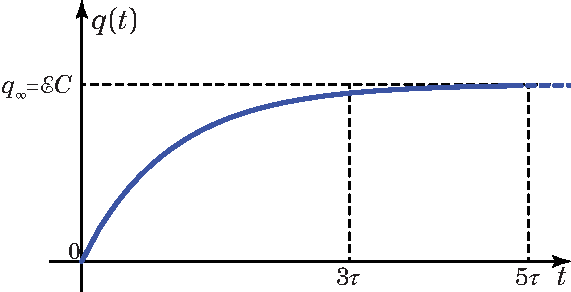
\includegraphics[width=0.85\textwidth]{images/chp5/chp5caricacondgraf1.pdf}
\end{center}
\paragraph{Tempo caratteristico del circuito RC}
L'andamento temporale della carica è dettato dal \textbf{tempo caratteristico del circuito RC}\index{tempo caratteristico!del circuito RC}:
\begin{equation}
	\tcboxmath[colback=yellowpastellow!30!white,drop fuzzy shadow, nobeforeafter, math upper, tcbox raise base, enhanced]{\tau=RC}
\end{equation}
Essa è una costante dimensionalmente pari ad una quantità temporale e quindi nel SI si misura in \textit{secondi}:
\begin{equation*}
	\left[\tau\right]=\left[R\right]\cdot\left[C\right]=\mathsf{M} \mathsf{L}^2  \mathsf{T}^{-3}\mathsf{I}^{-2}\cdot\mathsf{M}^{-1}\mathsf{L}^{-2}\mathsf{T}^4\mathsf{I}^2=\mathsf{T}
\end{equation*}
Come previsto, la carica dopo un tempo di carica \textit{infinito} è
\begin{equation}
	q_{\infty}=\mathcal{E}C
\end{equation}
Per un \textit{matematico}, ciò significherebbe che il condensatore non può mai caricarsi completamente; invece, per un \textit{fisico} questo si realizza - approssimando, chiaramente! - per un tempo tra $3\tau=3RC$ e $5\tau=5RC$. Infatti, si ha
\begin{align*}
q(3\tau)&=\mathcal{E}C\left(1-e^{-\nicefrac{3\Ccancel[red]{\tau}}{\Ccancel[red]{\tau}}}\right)=\num{0.950}\cdot\mathcal{E}C\\
q(5\tau)&=\mathcal{E}C\left(1-e^{-\nicefrac{5\Ccancel[red]{\tau}}{\Ccancel[red]{\tau}}}\right)=\num{0.993}\cdot\mathcal{E}C
\end{align*}
i quali sono valori \textit{molto} vicini al valore asintotico $q_{\infty}$ e che nella pratica possiamo assimilare ad esso.
\paragraph{Corrente nel circuito RC}
Per ottenere la corrente che attraversa il circuito ci basta considerare il flusso di corrente attraverso il condensatore - in poche parole, basta derivare $q(t)$ rispetto al tempo:
\begin{equation}
	\tcboxmath[colback=yellowpastellow!30!white,drop fuzzy shadow, nobeforeafter, math upper, tcbox raise base, enhanced]{I(t)=\dv{q(t)}{t}=\frac{\mathcal{E}}{R}e^{-\frac{t}{RC}}}
\end{equation}
\begin{center}
	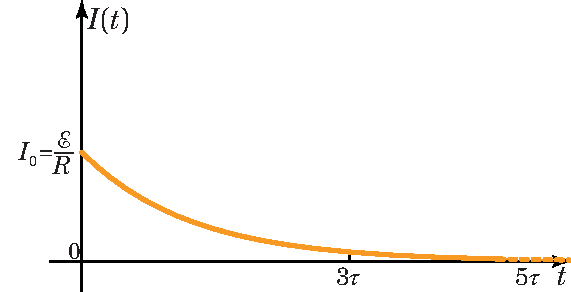
\includegraphics[width=0.8\textwidth]{images/chp5/chp5caricacondgraf2.pdf}
\end{center}
Come previsto, la corrente che percorre inizialmente il circuito è $\dfrac{\mathcal{E}}{R}$, mentre asintoticamente tende a zero.
\paragraph{Differenze di potenziali nel circuito RC}
Noto carica e corrente, i valori delle \ddp ai capi del resistore e del condensatore sono facili da ricavare:
\begin{empheq}[box=\tcmathboxgeneral]{align}
	V_C(t)&=\frac{q(t)}{C}=\mathcal{E}\left(1-e^{-\frac{t}{RC}}\right)\\
	V_R(t)&=RI(t)=\mathcal{E}e^{-\frac{t}{RC}}
\end{empheq}
\begin{minipage}{0.49\textwidth}
	\begin{center}
		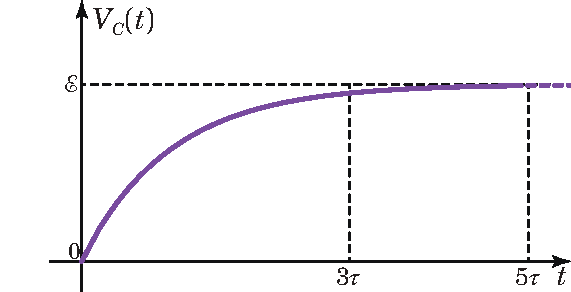
\includegraphics[width=1\textwidth]{images/chp5/chp5caricacondgraf3.pdf}
	\end{center}
\end{minipage}
\begin{minipage}{0.49\textwidth}
	\begin{center}
		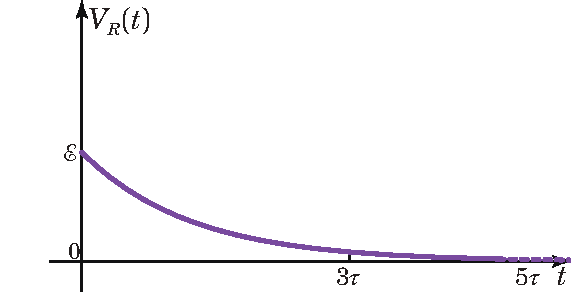
\includegraphics[width=1\textwidth]{images/chp5/chp5caricacondgraf4.pdf}
	\end{center}
\end{minipage}
Riprendendo quanto già detto, il voltaggio del condensatore aumenta al crescere del tempo di carica, mentre quello del resistore diminuisce.
\paragraph{Potenze ed energia nel circuito RC}
La \textit{potenza} erogata dal generatore è ovviamente dipendente dal tempo e vale
\begin{equation}
	\tcboxmath[colback=yellowpastellow!30!white,drop fuzzy shadow, nobeforeafter, math upper, tcbox raise base, enhanced]{P_{gen}(t)=\mathcal{E}I(t)=\frac{\mathcal{E}^2}{R}e^{-\frac{t}{RC}}}
\end{equation}
mentre quella dissipata del resistore è, in base all'effetto Joule,
\begin{equation}
	\tcboxmath[colback=yellowpastellow!30!white,drop fuzzy shadow, nobeforeafter, math upper, tcbox raise base, enhanced]{P_{R}(t)=I^2(t)R=\frac{\mathcal{E}^2}{R}e^{-\frac{2t}{RC}}}
\end{equation}
Noto che il lavoro per caricare il condensatore è $W=\dfrac{1}{2}V_Cq$, la potenza elementare relativa è la sua derivata temporale\footnote{Si vede, infatti che
\begin{equation*}
	P_{C}=\dv{W}{t}=\dv{t}\left(\frac{1}{2}V_Cq\right)=\frac{1}{2}\left(q\dv{V_C}{t}+V_C\dv{q}{t}\right)=\frac{1}{2}\left(q\dv{V_C}{t}+V_CI\right)
\end{equation*}
ed essendo $V_C=\dfrac{q}{C}$, allora $\dv{V_C}{t}=\dfrac{1}{C}\dv{q}{t}=\frac{I}{C}$ e quindi
\begin{equation*}
	P_{C}=\frac{1}{2}\left(q\frac{I}{C}+V_CI\right)=\frac{1}{2}\left(V_CI+V_CI\right)=V_CI
\end{equation*}}, ossia 
\begin{equation}
	P_{C}(t)=V_C(t)I(t)=\frac{\mathcal{E}^2}{R}e^{-\frac{t}{RC}}-\frac{\mathcal{E}^2}{R}e^{-\frac{2t}{RC}}=P_{gen}-P_{R}
\end{equation}
Ciò è coerente col \textit{principio di conservazione dell'energia}: l'energia immagazzinata (per unità di tempo) dal condensatore è ciò che \textit{rimane} dell'energia prodotta dal generatore dopo che parte di essa è stata dissipata sotto forma di calore dal resistore.\\
Sul lungo termine, l'energia prodotta dal generatore complessivamente è
\begin{equation*}
	W_{gen}=\int_{0}^{+\infty}P_{gen}(t)dt=\frac{\mathcal{E}^2}{R}\int_{0}^{+\infty}e^{-\frac{t}{RC}}=-\frac{\mathcal{E}^2}{\Ccancel[red]{R}}\Ccancel[red]{R}C\eval{e^{-\frac{t}{RC}}}_{0}^{+\infty}=\mathcal{E}^2C
\end{equation*}
\begin{equation}
	\tcboxmath[colback=yellowpastellow!30!white,drop fuzzy shadow, nobeforeafter, math upper, tcbox raise base, enhanced]{W_{gen}=\mathcal{E}^2C}
\end{equation}
mentre quella dissipata dal resistore è
\begin{equation*}
	W_{R}=\int_{0}^{+\infty}P_{R}(t)dt=\frac{\mathcal{E}^2}{R}\int_{0}^{+\infty}e^{-\frac{2t}{RC}}=-\frac{1}{2}\frac{\mathcal{E}^2}{\Ccancel[red]{R}}\Ccancel[red]{R}C\eval{e^{-\frac{2t}{RC}}}_{0}^{+\infty}=\frac{1}{2}\mathcal{E}^2C
\end{equation*}
\begin{equation}
	\tcboxmath[colback=yellowpastellow!30!white,drop fuzzy shadow, nobeforeafter, math upper, tcbox raise base, enhanced]{W_{R}=\frac{1}{2}\mathcal{E}^2C}
\end{equation}
\begin{observe}
	L'energia dissipata complessivamente dal resistore è indipendente dal valore della resistenza, ma è sempre la \textit{metà} di quanto produce il generatore di \fem.
\end{observe}
Per il \textit{principio di conservazione dell'energia}, il lavoro di carica del condensatore è pari a 
\begin{equation}
	W_{gen}=\frac{1}{2}\mathcal{E}^2C
\end{equation}
\paragraph{⋆ Processo di scarica}
Consideriamo ora un circuito, dotato di un interruttore inizialmente aperto, con un resistore $R$ e un condensatore $C$ di carica iniziale $q$, dotato di un interruttore inizialmente aperto.

\begin{center}		
	\begin{tikzpicture}[voltage dir=RP]
		\draw (0,0) -- (0,2.5)
		to [resistor, R=$R_1$, v=$V_R$] (2.5,2.5)
		to [capacitor, C=$C$, v=$V_C$] (2.5,0)
		to [switch, label=$t<0$, mirror] (0,0)
		-- (0,0.1);
		\draw (1,0) to[short, *-] (1,0);
	\end{tikzpicture}
	\begin{tikzpicture}[voltage dir=RP]
		\draw (0,0) -- (0,2.5)
		to [resistor, R=$R_1$, v=$V_R$] (2.5,2.5)
		to [capacitor, C=$C$, v=$V_C$] (2.5,0)
		-- (0,0) 
		-- (0,0.1);
		\draw (1,0) to[short, *-] (1,0);
		\node at (1.25,-0.5) {$t>0$};
		\node at (1.25,-0.6) {$ $};
	\end{tikzpicture}
\end{center}
La \ddp ai capi del condensatore è
\begin{equation*}
	V_0=V_C(0)=\frac{q}{C}
\end{equation*}
e l'energia elettrica immagazzinata è
\begin{equation*}
	U=\frac{q^2}{2C}
\end{equation*}
Al tempo $t=0$ viene chiuso l'interruttore: le cariche si muovono dall'armatura a potenziale maggiore a quella a potenziale minore, dando luogo ad un moto di cariche e, di conseguenza, ad una corrente elettrica
\begin{equation*}
	I=-\dv{q}{t}
\end{equation*}
dove il meno è dovuto al fatto che la carica \textit{diminuisce} nel tempo. In un generico istante $t>0$ la \ddp ai capi del condensatore è la stessa ai capi del resistore, e quindi si ha
\begin{align*}
	V_C&=\frac{q}{C}=V_R=RI=-R\dv{q}{t}\\
	\dv{q}{t}&=-\frac{q}{RC}
\end{align*}
Risolviamo questa \textit{equazione differenziale del prim'ordine} per descrivere la carica $q=q(t)$ del condensatore:
\begin{align*}
	\dv{q}{t}&=-\frac{q}{RC}\\
	\int_{q_0}^{q(t)}\frac{dq}{q}&=-\frac{1}{RC}\int_{0}^{t}dt\\
	\eval{\log{q}}_{q_0}^{q(t)}&=-\frac{1}{RC}\eval{t}_{0}^{t}\\
	\log{\frac{q(t)}{q_0}}&=-\frac{t}{RC}\\
	\frac{q(t)}{q_0}&=e^{-\frac{t}{RC}}
\end{align*}
\begin{equation}
	\tcboxmath[colback=yellowpastellow!30!white,drop fuzzy shadow, nobeforeafter, math upper, tcbox raise base, enhanced]{q(t)=q_0e^{-\frac{t}{RC}}=q_0e^{-\frac{t}{\tau}}}
\end{equation}
\begin{center}
	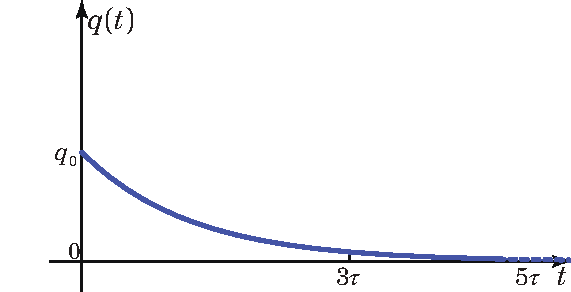
\includegraphics[width=0.85\textwidth]{images/chp5/chp5scaricacondgraf1.pdf}
\end{center}
Oltre alla carica, anche la \ddp di potenziale ai capi del condensatore e la corrente nel circuito diminuiscono esponenzialmente.
\begin{empheq}[box=\tcmathboxgeneral]{align}
	I(t)&=-\dv{q(t)}{t}=\frac{q_0}{RC}e^{-\frac{t}{RC}}=\frac{V_0}{R}e^{-\frac{t}{RC}}\\
	V_C(t)&=\frac{q(t)}{C}=\frac{q_0}{C}e^{-\frac{t}{RC}}
\end{empheq}
La \textit{potenza} dissipata del resistore è, in base all'effetto Joule,
\begin{equation}
	\tcboxmath[colback=yellowpastellow!30!white,drop fuzzy shadow, nobeforeafter, math upper, tcbox raise base, enhanced]{P_{R}(t)=I^2(t)R=\frac{V_0^2}{R}e^{-\frac{2t}{RC}}}
\end{equation}
mentre l'energia dissipata dal resistore è
\begin{equation*}
	W_{R}=\int_{0}^{+\infty}P_{R}(t)dt=\frac{V_0^2}{R}int_{0}^{+\infty}e^{-\frac{2t}{RC}}=-\frac{1}{2}\frac{V_0^2}{\Ccancel[red]{R}}\Ccancel[red]{R}C\eval{e^{-\frac{2t}{RC}}}_{0}^{+\infty}=\frac{1}{2}V_0^2C=\frac{q_0^2}{2C}
\end{equation*}
\begin{equation}
	\tcboxmath[colback=yellowpastellow!30!white,drop fuzzy shadow, nobeforeafter, math upper, tcbox raise base, enhanced]{W_{R}=\frac{1}{2}V_0^2C=\frac{q_0^2}{2C}}
\end{equation}
ossia è pari all0energia elettrostatica iniziale del condensatore.
\begin{observe}
	Si noti come il circuito RC, durante il processo di scarica, presenta comunque una corrente elettrica pur non avendo alcun generatore di \fem collegato.
\end{observe}